\documentclass[10pt]{article}

\usepackage{amsmath,amssymb,graphicx,booktabs}
\usepackage[a4paper,top=16mm,bottom=18mm,left=12mm,right=12mm]{geometry}
\usepackage[authoryear,round]{natbib}
\usepackage[T1]{fontenc}
\usepackage{newtxtext,newtxmath}
\usepackage{microtype}
\usepackage{xcolor}
\usepackage{xurl}
\usepackage{hyperref}

\setlength{\parindent}{1.2em}
\setlength{\parskip}{0pt}
\setlength{\columnsep}{6mm}
\setlength{\emergencystretch}{2em}
\pagestyle{plain}

\hypersetup{
  colorlinks=true,
  linkcolor=blue!50!black,
  citecolor=blue!50!black,
  urlcolor=blue!50!black,
  pdftitle={A single Einstein--Dilaton geometry linking hadron spectra, galaxy rotation curves, and cosmological growth},
  pdfauthor={Adrian Bohoyo},
  pdfsubject={Einstein--dilaton effective reconstruction and cross-domain readouts},
  pdfkeywords={Einstein--dilaton, holography, effective action, glueball spectrum, SPARC, cosmological growth}
}

\graphicspath{{../figures/}}
\newcommand{\Kphi}{K(\phi)}
\newcommand{\fsig}{f\sigma_8}
\newcommand{\LCDM}{\Lambda\mathrm{CDM}}
\newcommand{\dd}{\mathrm{d}}

\begin{document}
\sloppy
\twocolumn[
\begin{minipage}{\textwidth}
\begin{center}
{\LARGE\bfseries A single Einstein--Dilaton geometry linking hadron spectra,
galaxy rotation curves, and cosmological growth\par}
\vspace{0.9em}
{\large Adrian Bohoyo\par}
\vspace{0.25em}
{\small Systems Architect (R\&D), Monfragüe, Spain\par}
{\small ORCID: 0009-0003-1833-4519\par}
{\small \href{mailto:rydbergphotonic1@proton.me}{rydbergphotonic1@proton.me}\par}
\end{center}

\begin{abstract}
A corrected, geometry-preserving formulation is given for a frozen
five-dimensional Einstein--dilaton background used as a common computational
input for hadronic, galactic, cosmological, and laboratory readouts.  A
three-stage audit first derives and seals the field equations, then compares
the frozen trace with the previously declared canonical polynomial action, and
finally adjudicates the result in an independent coordinate representation.
The stored trace does not solve that polynomial system as labelled.  It is
shown, however, that the achieved warp and scalar profiles admit a healthy effective
completion
$S_{\rm eff}\propto\int\sqrt{-g}\bigl(R-\Kphi(\partial\phi)^2/2-V(\phi)\bigr)$.
The reconstructed kinetic function is strictly positive on the certified
radial interval, so the completion is equivalent to a canonical scalar by
field redefinition.  The warp and scalar profiles are preserved to
$2.04\times10^{-6}$ and $8.54\times10^{-8}$, respectively, while the complete
field equations close at normalized floating-point residuals below
$8\times10^{-17}$.  The deformation used by the observational arms is recovered
with correlation $0.999999905$ and rms difference $6.88\times10^{-4}$.
On a separately declared compact-interval probe branch, the geometry-fixed
trace carrier yields the normalized matter coupling
$\beta_n=\sqrt{I_g/3}\,f_n$.  Explicitly selected Neumann endpoints give
$\beta_0=0.0542901$ and a conditional unscreened scalar-force fraction
$2\beta_0^2=5.89483\times10^{-3}$; the corresponding massless scalar-tensor
branch is incompatible with Solar-System bounds and is not a viable discovery
claim.  The six positive modes define a correlated material-force template,
but their ranges still require a physical length.  No observational input
enters that derivation; the interval interpretation and boundary/junction
completion remain assumptions.  A Liouville transformation shows that this
carrier and the gauge-invariant scalar operator are the same local degree of
freedom under different boundary and physical interpretations, not two towers
to be added.
An exhaustive NN/ND/DN/DD endpoint audit then tests the simplest boundary
alternatives without observational input.  NN retains the excluded massless
mode; ND produces an independently verified UV-coupled ultralight mode with
$m\ell=0.00274476$ and $\beta_{\rm UV}=0.0542910$; and UV Dirichlet branches
decouple an exact point probe.  Thus changing one endpoint is not a
data-independent rescue, and a physical boundary action remains necessary.
The existing scalar-spectrum value $m_1/m_0=1.5455$ is retained as an
operator-level diagnostic pending recomputation on a prospectively frozen
analytic completion.  The SPARC result is reported as a global in-sample
calibration against its baryonic Newtonian baseline with no per-galaxy
parameters, and the growth and laboratory arms
as explicit dictionary-dependent projections.  A corrected Ricci audit and a
Wilson-scale audit further show that the legacy clock used a mislabeled radial
derivative and that the stored ``Wilson-loop'' value is an endpoint proxy with
external normalization, not a measured area law.  This revision therefore
preserves the operational shared-background instrument while separating its
verified computational content, one conditional matter interface, and the
remaining forward predictions that require additional interface actions or
held-out validation.
The electromagnetic audit exposes and corrects a radial-gauge error: the
historical numerical kernel treated the stored domain-wall grid as a conformal
coordinate.  A covariant bulk-Maxwell reduction instead gives the same
probability measure in both gauges, an action-derived scalar--photon vertex,
and a photon Kaluza--Klein comb.  Together with the scalar carrier, this forms
a correlated two-sector spectral fingerprint with one still-unfixed physical
length.  Its central coefficients require no observational fit, but photon
localization, boundary action, source, scale, and atomic sensitivity remain
unselected; it is therefore a conditional prediction rather than a detection.
Finally, a retrospective
galaxy-level split finds that a train-only five-parameter SPARC refit improves
on baryons-only Newton but is substantially worse than a train-fitted
one-parameter radial-acceleration baseline.  A four-bin DESI DR1 marginal
growth diagnostic gives $\chi^2=2.692$ for the frozen dictionary and $2.419$
for matched $\LCDM$, providing no preference for the former.
\end{abstract}

\noindent\textbf{Key words:} gravitation -- holography -- galaxies: kinematics
and dynamics -- cosmology: large-scale structure of Universe -- methods:
numerical
\end{minipage}
\vspace{1.2em}
]

\section{Introduction}

Einstein--scalar domain walls provide a controlled language for holographic
renormalization-group flows and, with an appropriate infrared completion, for
confining Yang--Mills phenomenology \citep{DeWolfe2000,Gursoy2008,Gursoy2011}.
The project studied here uses one frozen bulk profile as a shared input for a
gauge-invariant scalar fluctuation operator, a global SPARC readout, a
cosmological-growth dictionary, and versioned single-arm response operators.
That common dependency and the accompanying machine-readable artefacts are an
operational achievement: every arm can be rerun against the same frozen arrays.

Reproducibility of a common input is not, by itself, a derivation of all
interfaces from one action.  The stronger claim requires two separate checks.
First, the bulk arrays must solve the field equations associated with the
declared action and gauge.  Secondly, mappings from the holographic radius to a
galaxy radius, cosmological redshift, or laboratory time must either follow
from an explicit interface action or be identified as phenomenological
dictionaries.

This revision performs those checks without discarding the achieved geometry.
Section~\ref{sec:action} derives the complete bulk equations.  Section~\ref{sec:audit}
records the three-stage consistency audit and identifies a preconditioning
label mismatch.  Section~\ref{sec:effective} reconstructs a positive effective
kinetic function and potential that support the frozen profiles.
Section~\ref{sec:probe} derives one explicitly conditional probe-matter
interface without observational calibration.  The remaining sections retain
the established numerical readouts with corrected evidential labels.  No
simultaneous multi-arm inversion or laboratory detection is claimed.

\section{Effective Einstein--dilaton background}
\label{sec:action}

Signature $(-,+,+,+,+)$ is used together with the effective action
\begin{equation}
 S_{\rm eff}=\frac{1}{2\kappa_5^2}\int\dd^5x\sqrt{-g}
 \left[R-\frac12\Kphi(\partial\phi)^2-V(\phi)\right].
 \label{eq:action}
\end{equation}
The canonical model is the special case $K=1$.  Variation gives
\begin{align}
 R_{MN}&=\frac12K\,\partial_M\phi\partial_N\phi+\frac13g_{MN}V,\label{eq:einstein}\\
 K\nabla^2\phi+\frac12K_{,\phi}(\partial\phi)^2&=V_{,\phi}.
 \label{eq:scalarcov}
\end{align}

In domain-wall gauge,
\begin{equation}
 \dd s^2=e^{2A(u)}\eta_{\mu\nu}\dd x^\mu\dd x^\nu+\dd u^2,
 \qquad \phi=\phi(u),
 \label{eq:domainwall}
\end{equation}
these equations reduce to
\begin{align}
 A''&=-\frac16K\phi'^2,\label{eq:warp}\\
 12A'^2-\frac12K\phi'^2+V&=0,\label{eq:constraint}\\
 K(\phi''+4A'\phi')+\frac12K_{,\phi}\phi'^2&=V_{,\phi}.
 \label{eq:scalar}
\end{align}
Primes in Eqs.~(\ref{eq:warp})--(\ref{eq:scalar}) denote $\dd/\dd u$.
The constraint alone is not a substitute for the two dynamical equations.

For comparison in conformal gauge, define $\dd z/\dd u=e^{-A}$.  The metric is
$\dd s^2=e^{2A(z)}(\eta_{\mu\nu}\dd x^\mu\dd x^\nu+\dd z^2)$ and the equations
transform covariantly.  Pure AdS has constant $A_u=\pm L^{-1}$ in domain-wall
gauge but $A_z=-z^{-1}$ in the usual conformal orientation.  These reference
derivatives must not be mixed.

\subsection{Constraint propagation and matter sources}

For the canonical vacuum system, differentiating
$H=12A'^2-\phi'^2/2+V$ and inserting the dynamical equations gives $H'=0$.
If a density is added only through
$A''=-\phi'^2/6-\kappa\rho$ while the vacuum constraint is retained, then
\begin{equation}
 H'=-24\kappa A'\rho.
 \label{eq:constraintdrift}
\end{equation}
A consistent matter source therefore requires its action, conserved stress
tensor, and corresponding constraint contribution.  Equation~(\ref{eq:constraintdrift})
is the reason the old sourced polynomial interpretation cannot be retained
unchanged.

\section{Three-stage audit of the frozen trace}
\label{sec:audit}

The trace contains 1999 samples over the stored coordinate range
$[0.01,2]$.  The audit was separated into: (i) direct derivation and sealing of
the equations and thresholds; (ii) comparison with hash-frozen candidate
outputs; and (iii) independent integration and coordinate-gauge adjudication.
Input hashes and thresholds are included in the public audit artefacts.

An independent positive control is provided by
\begin{equation}
 W(\phi)=\frac6L+\frac{\phi^2}{2L},\qquad
 V=\frac12W_{,\phi}^2-\frac13W^2,
\end{equation}
which gives
\begin{equation}
 V=-\frac{12}{L^2}-\frac{3\phi^2}{2L^2}-\frac{\phi^4}{12L^2}
\end{equation}
and the exact flow
\begin{equation}
 \phi=\phi_0e^{(u-u_0)/L},\quad
 A=A_0-\frac{u-u_0}{L}-\frac{\phi^2-\phi_0^2}{24}.
\end{equation}
It has $m^2L^2=-3$, above the $AdS_5$ Breitenlohner--Freedman bound
\citep{Breitenlohner1982}.  Independent second-order integration agrees with
the exact solution to $4.92\times10^{-14}$; the largest conformal-gauge
residual is $3.55\times10^{-15}$.

Table~\ref{tab:audit} reports the same tests on the frozen trace.  Both the
literal stored polynomial sign and the intended BF-mass sign fail the sealed
criteria.  The previously reported maximum raw constraint residual, 1.81, is
therefore not treated as a harmless diagnostic.

\begin{table}
 \centering
 \caption{Equation-level audit of the frozen trace.  Values are normalized
 residuals; all listed tests fail their sealed criterion.}
 \label{tab:audit}
 \begin{tabular}{lccc}
  \toprule
  Metric & Literal & BF sign & Criterion\\
  \midrule
  $\phi$ kinematic rms & 0.3139 & 0.3139 & $\leq0.01$\\
  $A$ kinematic rms & 0.4615 & 0.4615 & $\leq0.01$\\
  Constraint p95 & 0.03852 & 0.03851 & $\leq0.001$\\
  Scalar EOM rms & 0.3220 & 0.3543 & $\leq0.01$\\
  Sourced warp EOM rms & 0.8903 & 0.8903 & $\leq0.01$\\
  \bottomrule
 \end{tabular}
\end{table}

The cause is identifiable.  The original numerical preconditioner rescales
the state, evaluates an untransformed right-hand side, and then reverses the
scaling.  Consequently the stored columns satisfy approximately
\begin{equation}
 A_{,u}\simeq u(dA)_{\rm stored},\qquad
 \phi_{,u}\simeq (d\phi)_{\rm stored}/u,
 \label{eq:storedrelation}
\end{equation}
rather than being direct derivative columns.  This is a provenance and label
error, not evidence that the smooth warp geometry itself must be discarded.

The Bessel-based holonomic proxy in the previous version remains useful as a
compact fit, but it imposes only Eq.~(\ref{eq:constraint}).  Its normalized
constraint residual is $1.48\times10^{-16}$ whereas its scalar and warp
residuals are 0.9546 and 0.9494.  That construction is therefore moved to the
status of a descriptive proxy and is not used as the bulk action.

\section{Geometry-preserving effective completion}
\label{sec:effective}

For monotonic $\phi(u)$ and $A''(u)<0$, Eqs.~(\ref{eq:warp}) and
(\ref{eq:constraint}) can be inverted:
\begin{equation}
 K(\phi(u))=-\frac{6A''(u)}{\phi'(u)^2},\qquad
 V(\phi(u))=-3A''(u)-12A'(u)^2.
 \label{eq:inverse}
\end{equation}
The scalar equation then follows from the derivative of the constraint wherever
$\phi'\neq0$.  This is a geometry-preserving inverse completion: it asks which
action supports the achieved profiles instead of replacing those profiles with
the audit control solution.

Quintic smoothing splines remove sub-micro-scale integration noise.  Ten
samples at each endpoint are excluded because high-order derivatives are
boundary sensitive.  The certified interval is
\begin{equation}
 0.010233\leq u\leq1.980981.
\end{equation}
On this interval, the fit changes $A$ by at most $2.04\times10^{-6}$ and
$\phi$ by at most
$8.54\times10^{-8}$.  The kinetic function obeys
\begin{equation}
 8.55\leq K(\phi)\leq9.39\times10^6,
\end{equation}
and is strictly positive at every certified sample.  The wide range signals a
poor normalization of the stored scalar near the ultraviolet endpoint, but not
a kinetic ghost.

Defining a canonical scalar by
\begin{equation}
 \chi'(u)=\sqrt{-6A''(u)}
 \label{eq:canonicalfield}
\end{equation}
gives an equivalent canonical representation.  Table~\ref{tab:completion}
shows closure in both field variables.

\begin{table}
 \centering
 \caption{Certificate for the effective completion.}
 \label{tab:completion}
 \begin{tabular}{lr}
  \toprule
  Quantity & Value\\
  \midrule
  Non-canonical warp max residual & $2.22\times10^{-16}$\\
  Constraint max residual & $7.11\times10^{-15}$\\
  Non-canonical scalar normalized rms & $7.58\times10^{-17}$\\
  Canonical warp max residual & $4.44\times10^{-16}$\\
  Canonical scalar max residual & $1.07\times10^{-14}$\\
  \bottomrule
 \end{tabular}
\end{table}

The operational deformation is also recovered.  Equation~(\ref{eq:storedrelation})
turns the stored expression $-u(dA)_{\rm stored}-1$ into the domain-wall
quantity
\begin{equation}
 \delta_{\rm eff}(u)=-A'(u)-1\qquad(L=1).
 \label{eq:deltaeff}
\end{equation}
Its correlation with the stored deformation is 0.999999905, with rms difference
$6.88\times10^{-4}$.  The shared observational input is therefore preserved to
high precision.

\begin{figure*}
 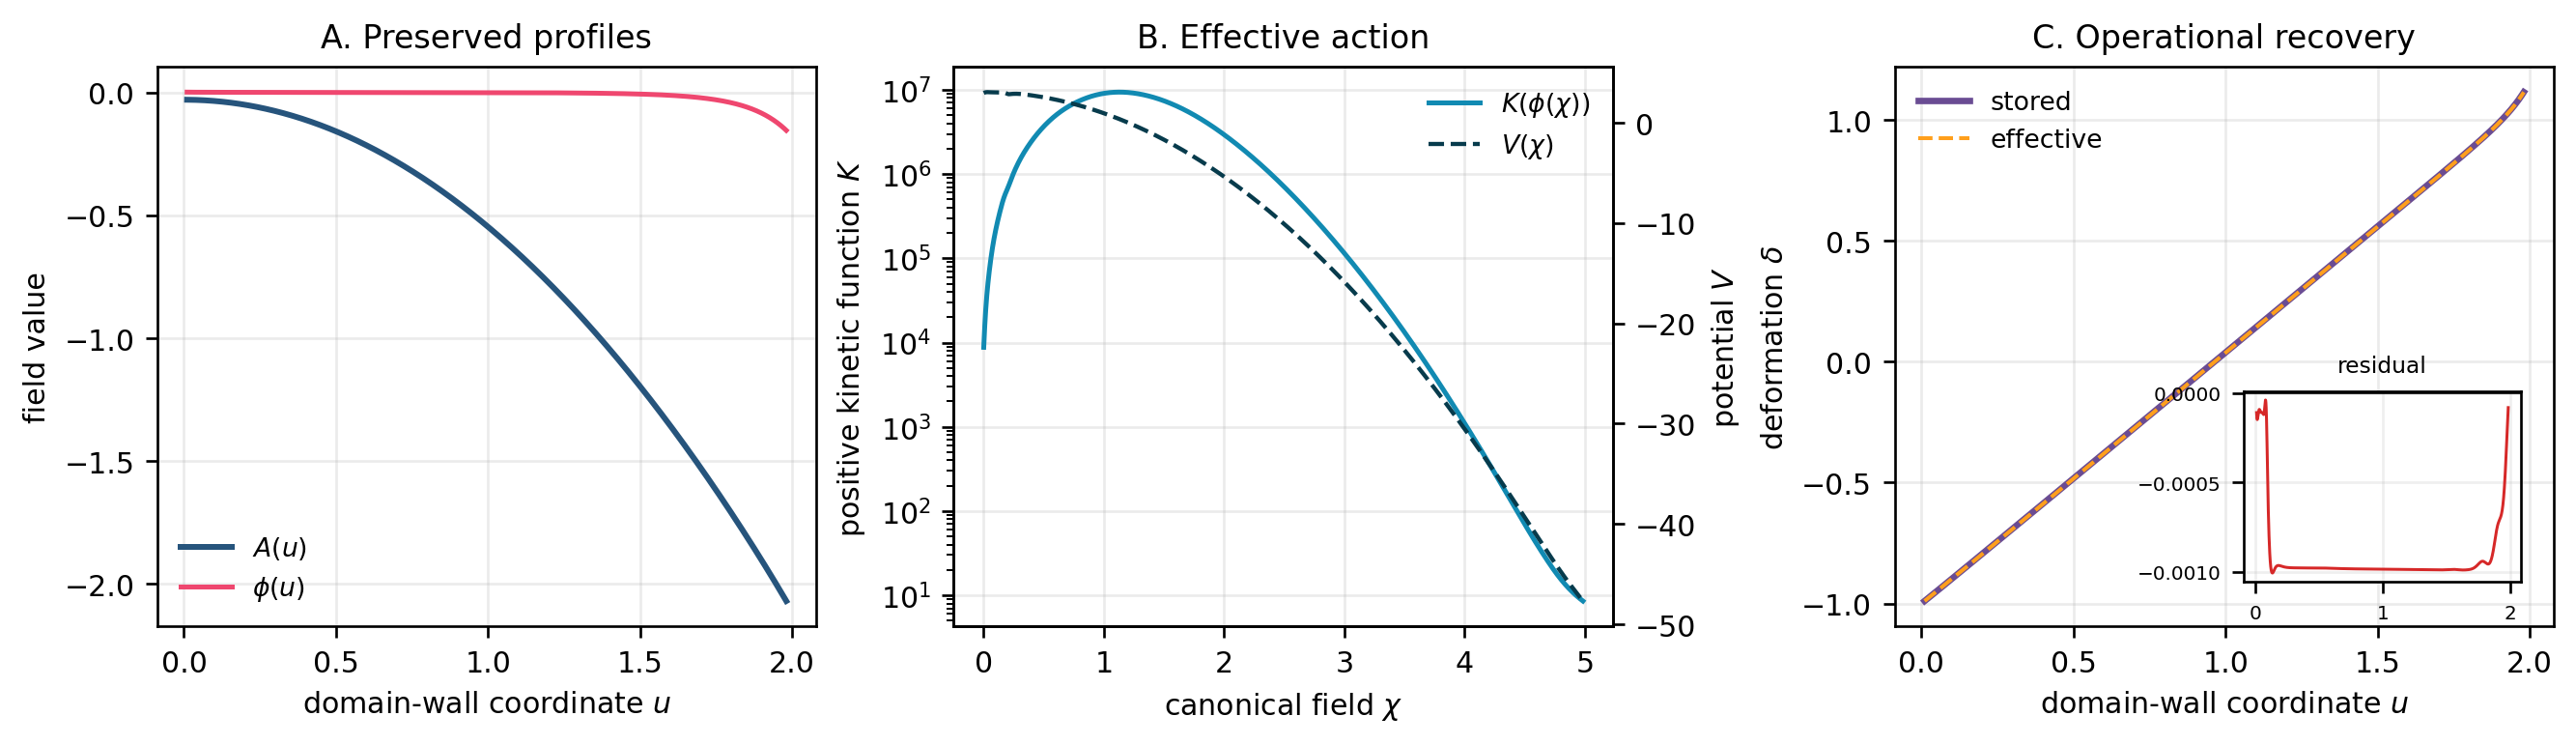
\includegraphics[width=\textwidth]{fig_effective_reconstruction.png}
 \caption{Geometry-preserving effective completion.  Left: reconstructed warp
 and scalar profiles on the certified interval.  Centre: positive kinetic
 function and potential in canonical field coordinates.  Right: stored and
 reconstructed operational deformations and their residual.}
 \label{fig:effective}
\end{figure*}

\section{Conditional compact-interval matter interface}
\label{sec:probe}

The corrected bulk fixes a healthy local scalar carrier, but a holographic
radial coordinate is not automatically an extra physical dimension.  A blind
forward benchmark is obtained by adding six explicit assumptions: one physical
copy of the certified interval; a consistent
Gibbons--Hawking--York/background/junction completion with no additional
localized quadratic trace term; selected Neumann endpoints; probe Standard
Model matter localized on a fixed slice; no brane bending or backreaction; and
induced-metric coupling only at tree level.  These assumptions are not selected
by the frozen trace.

Let $u_{\rm phys}=\ell u$ and define
\begin{equation}
 \epsilon=-\frac{A''}{A'^2}>0,\qquad
 p=e^{4A}\epsilon,\qquad w=e^{2A}\epsilon,
 \label{eq:carrierweights}
\end{equation}
where the ratio defining $\epsilon$ is invariant under the constant rescaling
from $u$ to $u_{\rm phys}$.  The local transverse-trace action, with the
normalization mapped from \citet{Arutyunov2000}, is
\begin{equation}
 S_h^{(2)}=-\frac{3\ell}{128\kappa_5^2}\int\dd^4x\,\dd u
 \left[w\eta^{\mu\nu}\partial_\mu h\partial_\nu h
 +\frac{p}{\ell^2}(h')^2\right].
 \label{eq:traceaction}
\end{equation}
That calculation supplies the local quadratic normalization; it does not
supply the compactification or the endpoint conditions used here.

With $p f_n'|_{\rm UV,IR}=0$, the dimensionless modes obey
\begin{align}
 -(p f_n')'&=\mu_n^2 w f_n, &
 \int\dd u\,w f_nf_m&=\delta_{nm},\label{eq:probesl}\\
 h(x,u)&=\sum_n q_n(x)f_n(u), &
 \varphi_n&=\frac{\sqrt{3\ell}}{8\kappa_5}q_n .
 \label{eq:probecanonical}
\end{align}
The physical trace-carrier masses are $M_n^{(h)}=\mu_n/\ell$.  This tower is
not an additional scalar tower independent of the $\zeta$ operator.  To see
this, introduce the conformal coordinate $\dd z_c=e^{-A}\dd u$ and
$s=e^{3A}\epsilon$.  Equation~(\ref{eq:probesl}) becomes
\begin{equation}
 -(s f_{n,z_c})_{,z_c}=\mu_n^2s f_n.
\end{equation}
Writing $\Psi_n=e^Bf_n$ with
\begin{equation}
 B=\frac12\log s=\frac32A+\frac12\log\epsilon
  =\frac32A+\log|X|+\mathrm{const},
 \qquad X=\frac{\chi'}{3A'},
\end{equation}
gives
\begin{equation}
 [-\partial_{z_c}^2+B'^2+B'']\Psi_n=\mu_n^2\Psi_n.
 \label{eq:liouvilleequivalence}
\end{equation}
This is the local gauge-invariant scalar operator.  The present Neumann
compactification, the stored Dirichlet--Neumann calculation, and their use of
canonical $\chi$ versus stored $\phi$ do not impose the same physical boundary
problem, so their numerical spectra need not agree.  They nevertheless describe
one scalar degree of freedom and cannot be double counted.  In the holographic
reading $u$ is an RG coordinate and the poles are composite; in the compact
reading it is a physical interval and the modes are four-dimensional scalars.

For a conserved probe stress tensor, the longitudinal trace-sector field
decouples and the transverse trace contributes
\begin{equation}
 \delta S_m=\int\dd^4x\sqrt{-g}\,\frac{hT}{8}
 =\sum_n\int\dd^4x\sqrt{-g}\,
 \frac{\beta_n}{M_{\rm Pl}}\varphi_nT .
\end{equation}
Tensor reduction on the same interval gives
\begin{equation}
 M_{\rm Pl}^2=\frac{\ell I_g}{\kappa_5^2},\qquad
 I_g=\int\dd u\,e^{2A},
\end{equation}
and therefore
\begin{equation}
 \boxed{\ \beta_n(u_m)=\sqrt{\frac{I_g}{3}}\,f_n(u_m)\ }.
 \label{eq:betaderived}
\end{equation}
The unknown $\kappa_5$ and the interval length cancel from the dimensionless
coupling, although $\ell$ remains necessary to fix every nonzero force range.

The blind numerical reduction gives $I_g=0.8079601$ and $I_w=91.37501$.
The Neumann zero mode is $f_0=I_w^{-1/2}$, so
\begin{equation}
 \beta_0=\sqrt{\frac{I_g}{3I_w}}=0.0542901,
 \qquad 2\beta_0^2=5.89483\times10^{-3}.
 \label{eq:zeroforce}
\end{equation}
If this massless branch survives the boundary completion, two unscreened
nonrelativistic bodies have
\begin{equation}
 V_{12}(r)=-\frac{G_Nm_1m_2}{r}\left(1+2\beta_0^2\right).
\end{equation}
Thus the scalar term is 0.589 per cent of the tensor Newtonian term in this
benchmark.  Under the standard universal massless scalar-tensor mapping it
would give
\begin{equation}
 \gamma=\frac{1-2\beta_0^2}{1+2\beta_0^2}=0.988279,
\end{equation}
whereas Cassini found $\gamma-1=(2.1\pm2.3)\times10^{-5}$
\citep{Bertotti2003}.  The massless unscreened Neumann branch is therefore
excluded.  A different boundary sector may lift or remove the zero mode, but
it must be specified prospectively and its complete spectrum recomputed.

The computed dimensionless tower is
\begin{align}
 (\mu_0,\ldots,\mu_3)&=(0,0.913899,1.541695,2.133778),\\
 (\mu_4,\ldots,\mu_6)&=(2.728899,3.336654,3.954473),
\end{align}
with UV-slice couplings
\begin{align}
 (\beta_0,\beta_1,\beta_2)&=(0.0542901,0.000705106,0.00155651),\\
 (\beta_3,\beta_4)&=(0.00233763,0.00282007),\\
 (\beta_5,\beta_6)&=(0.00306861,0.00320280).
\end{align}
The finite-element result passes mesh, orthonormality, residual, and zero-mode
checks; a separate shooting solve provides the independent numerical check.

For the six positive modes of the current Neumann basis,
$\alpha_n=2\beta_n^2$ sums to $7.20230\times10^{-5}$ and the correlated mass
ratios are
\begin{equation}
 1:1.686942:2.334807:2.985996:3.651009:4.327036.
\end{equation}
For $x=r/\ell$ they define the material-force templates
\begin{align}
 \frac{a_\varphi}{a_N}&=\sum_{n>0}\alpha_n(1+\mu_nx)e^{-\mu_nx},\\
 \frac{|\partial_r a_\varphi|}{|\partial_r a_N|}
 &=\sum_{n>0}\alpha_n\left(1+\mu_nx+\frac{\mu_n^2x^2}{2}\right)e^{-\mu_nx}.
 \label{eq:materialtemplate}
\end{align}
A mechanical mode with angular frequency $\omega_m$ and quality factor $Q$
then responds to a source-modulated differential acceleration as
\begin{equation}
 |\Delta x(\Omega)|=\frac{|\Delta a(\Omega)|}
 {\sqrt{(\omega_m^2-\Omega^2)^2+(\Omega\omega_m/Q)^2}}.
 \label{eq:mechanicaltransfer}
\end{equation}
Equations~(\ref{eq:materialtemplate})--(\ref{eq:mechanicaltransfer}) are a
transfer law, not a predicted signal: a source trajectory, $\ell$, detector
geometry, elastic response, noise, and mode occupation must still be supplied.

\begin{figure*}
 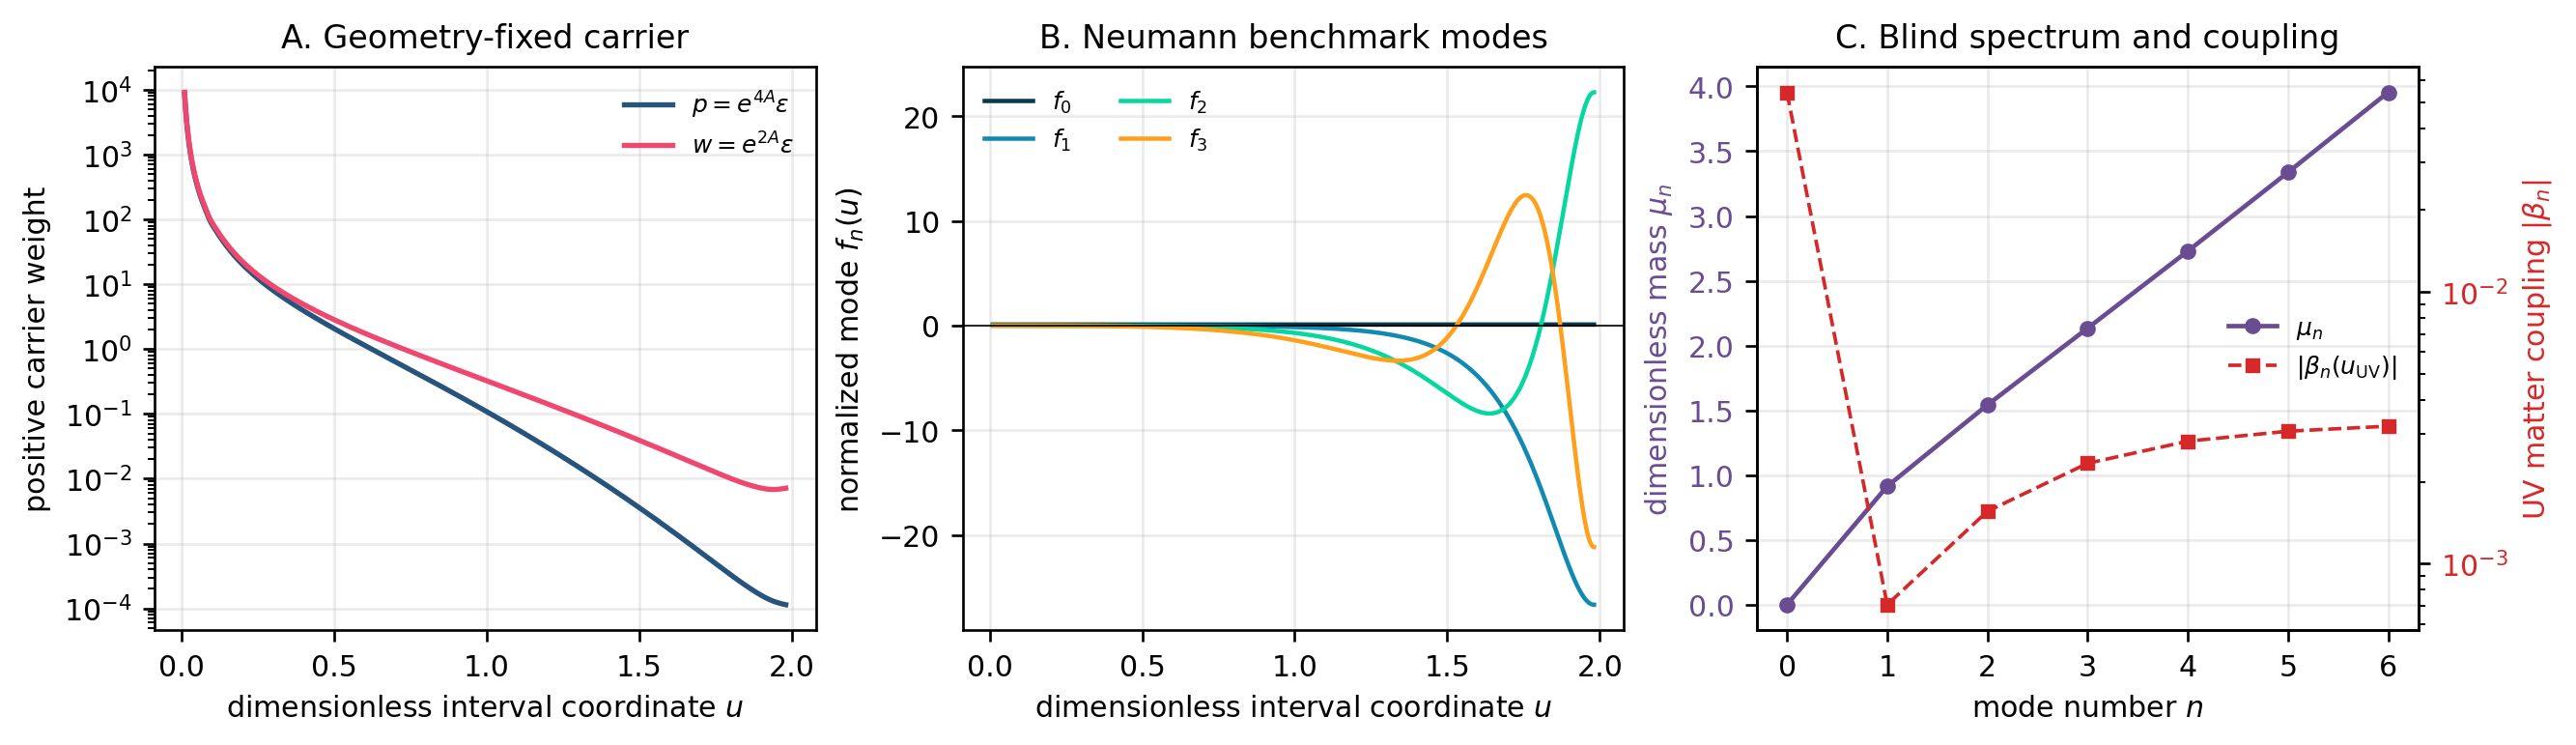
\includegraphics[width=\textwidth]{fig_minimal_probe_completion.png}
 \caption{Blind conditional matter completion.  Left: positive carrier
 weights fixed by the reconstructed geometry.  Centre: normalized Neumann
 benchmark modes.  Right: dimensionless trace-carrier masses and UV-slice
 matter couplings.  No observational residual or historical fitted coupling
 enters this calculation.}
 \label{fig:probecompletion}
\end{figure*}

For a Maxwell field localized on a four-dimensional slice,
$T_{\rm EM}=0$ and classical Weyl invariance gives no independent local
$\varphi_nF_{\mu\nu}F^{\mu\nu}$ vertex from the conformal induced metric.
This statement does not apply to a photon propagating through the fifth
dimension: its action also samples the perturbed radial lapse, whose
constraint-generated coupling is derived below.  A universal rescaling of all
masses does not by itself change leading clock-frequency ratios, and anomaly
or non-universal coefficients remain separate possible channels
\citep{Damour2010}.

\section{Data and evaluation protocol}

Table~\ref{tab:preservation} records the numerical cross-check against the
original PDF.  The values are retained; only their evidential interpretation
is tightened.  In particular, the original SPARC analysis was not benchmarked
against state-of-the-art dark-matter or modified-gravity fits.  Its declared
comparator was the baryonic Newtonian baseline under the same evaluation
protocol, and that comparison scope is not broadened here.

\begin{table*}
 \centering
 \caption{Cross-check of the principal numerical results against the original
 PDF.  ED/Newton denotes the ED-anchored and baryonic Newtonian readouts;
 dict/$\LCDM$ denotes the dictionary model and its matched flat-$\LCDM$
 reference.}
 \label{tab:preservation}
 \begin{tabular}{llll}
  \toprule
  Quantity & Original PDF & Revision & Evidential status\\
  \midrule
  Stored scalar ratio & $1.5455$ & $1.5454665$ & operator diagnostic\\
  IR scale proxy & $0.203\,{\rm GeV}^2$; $451\,{\rm MeV}$; $1.60\,{\rm GeV}$
    & unchanged & external normalization\\
  SPARC ranking medians (ED/Newton) & $1.86/1.93$ & $1.862/1.928$ & in-sample\\
  SPARC uncertainty medians (ED/Newton) & $831/906$ & $831/906$ & in-sample\\
  SPARC wins & $150/175$; $149/175$ & unchanged & same two metrics\\
  BOSS covariance $\chi^2$ (dict/$\LCDM$) & $2.266/2.443$ & unchanged
    & statistically indistinguishable\\
  High-$z$ growth shift & $\simeq-12$ per cent & unchanged
    & composite-dictionary prediction\\
  \bottomrule
 \end{tabular}
\end{table*}

\subsection{SPARC rotation curves}

SPARC provides 175 galaxies with $3.6\,\mu$m photometry, gas contributions,
and resolved rotation curves \citep{Lelli2016}.  The final model curve does not
read the observed velocity $v_{\rm obs}$ during forward evaluation.  Its five
global fitted parameters were, however, selected by differential evolution on the
same 175 curves.  The present result is therefore described as a global
\emph{in-sample calibration with no per-galaxy parameters}, not as a held-out
prediction.
The frozen global vector is
\begin{align}
 {\cal A}&=0.13983,& n&=2.21605,& m&=1.20433,\\
 \gamma&=0.23356,& \Sigma_0&=0.60488.
\end{align}

The original ranking loss is retained for exact reproducibility,
\begin{equation}
 {\cal L}_{\rm rank}=\sum_i
 \frac{[v_{\rm model}(r_i)-v_{\rm obs}(r_i)]^2}
 {v_{\rm obs}(r_i)^2+(1\,\mathrm{km\,s^{-1}})^2},
 \label{eq:rankloss}
\end{equation}
but is no longer denoted $\chi^2$ because its denominator is not an
observational variance.  The conventional uncertainty-weighted statistic is
reported separately.

\subsection{Growth and BOSS DR12}

The cosmological arm uses the explicit dictionary
\begin{equation}
 z_{\rm trace}=1+z_{\rm cos},\qquad N=-\ln z_{\rm trace}.
 \label{eq:growthdict}
\end{equation}
It is not derived from a compactification or a four-dimensional FRW action.
Predictions that use Eq.~(\ref{eq:growthdict}) are consequently labelled
dictionary-dependent.  The comparison uses the BOSS DR12 covariance at
$z=\{0.38,0.51,0.61\}$ \citep{Alam2017} and a matched Planck-2018 flat-$\LCDM$
reference with $\Omega_{m0}=0.315$, $H_0=67.4\,{\rm km\,s^{-1}\,Mpc^{-1}}$,
and $\sigma_{8,0}=0.811$ \citep{Planck2020}.

\section{Gauge-invariant scalar operator}

For a self-adjoint fluctuation problem,
\begin{equation}
 -(p\psi')'+q\psi=\lambda w\psi,
 \label{eq:SL}
\end{equation}
normalizable solutions with declared ultraviolet and infrared boundary
conditions define a discrete finite-domain spectrum.  The stored scalar
channel uses a Schrödinger potential $V_\zeta=B'^2+B''$, with
$B=3A/2+\log X$, Dirichlet ultraviolet and Neumann infrared conditions.

\begin{figure}
 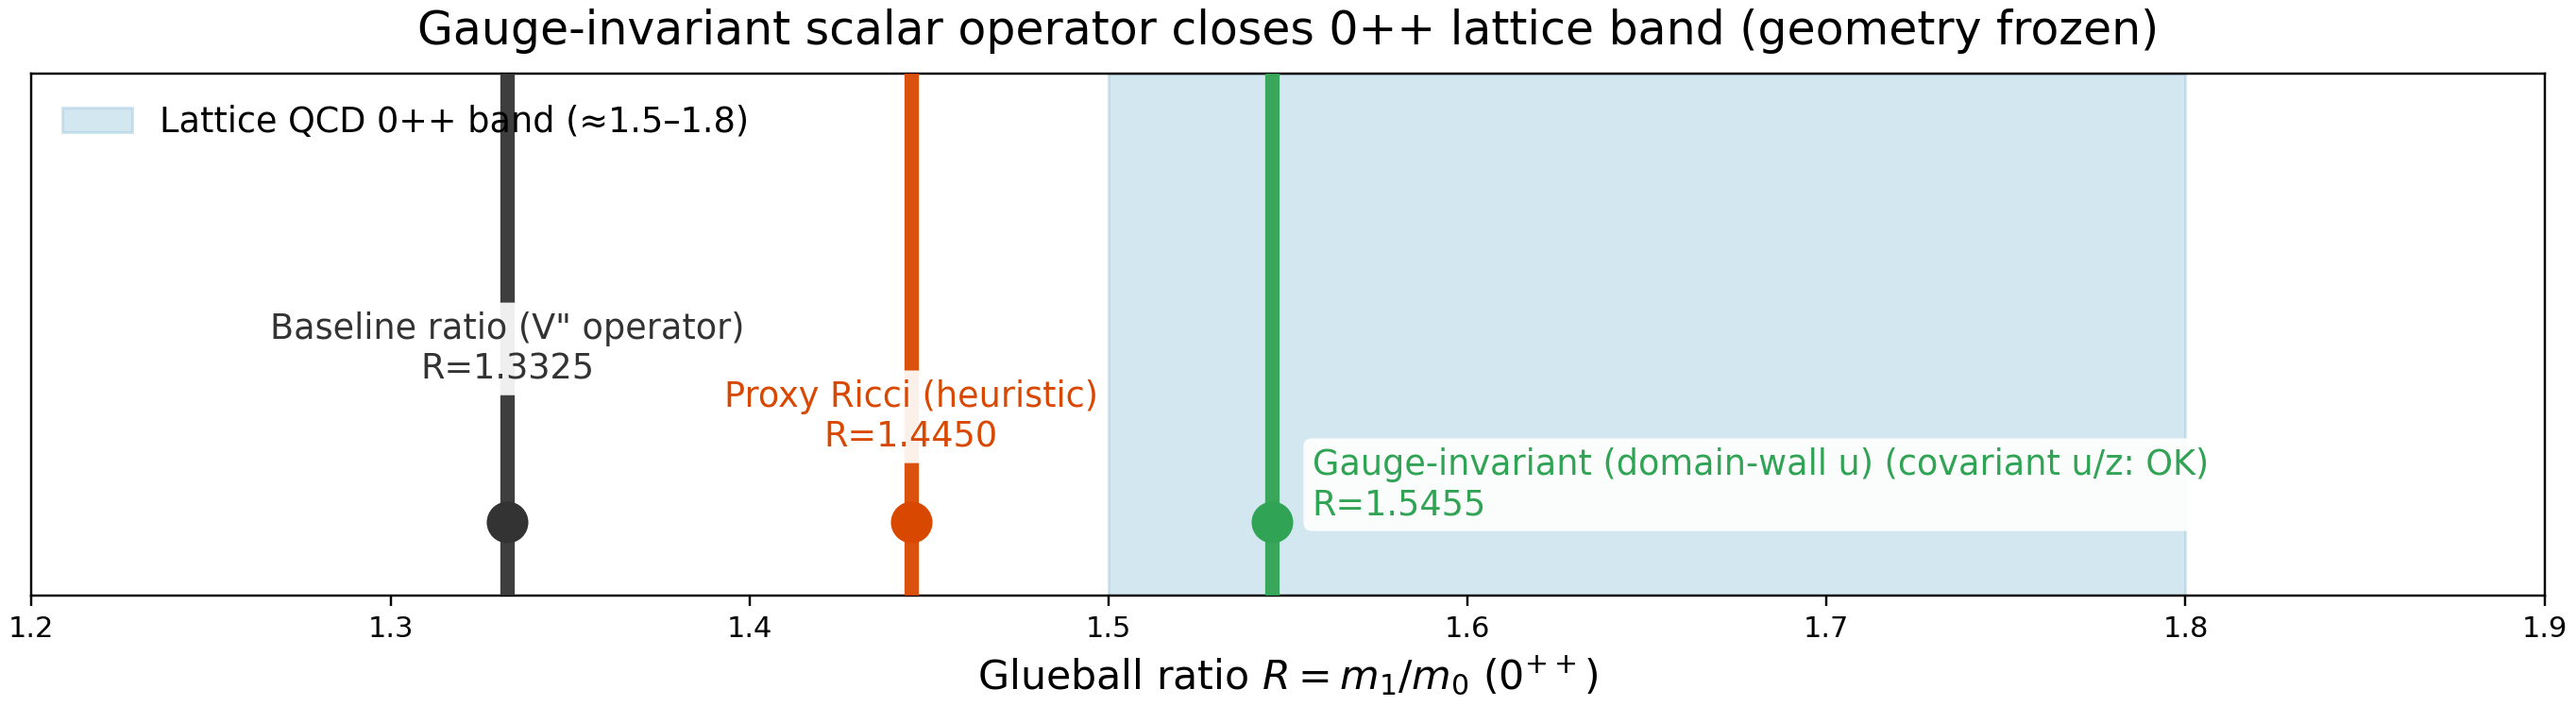
\includegraphics[width=\columnwidth]{glueball_ratio.png}
 \caption{Stored scalar $0^{++}$ operator ratio on the frozen profile.  In this
 revision $m_1/m_0=1.5455$ is retained as a reproducible operator diagnostic;
 it is not yet promoted to a physical glueball prediction of the reconstructed
 effective action.}
 \label{fig:glueball}
\end{figure}

The operator calculation gives
\begin{equation}
 (m_1/m_0)_{\rm stored}=1.5454665
\end{equation}
and agrees between its two covariantly transformed numerical realizations at
the $10^{-7}$ level.  This establishes internal coordinate consistency of the
stored operator calculation.  A physical glueball claim additionally requires
recomputation using the canonical field $\chi$, a confining infrared
completion, normalizability, and prospectively fixed boundary conditions
\citep{Gursoy2008,Gursoy2011,Morningstar1999}.
The stored value is compatible with the broad early estimate $1.54(11)$ of
\citet{Morningstar1999}, but the modern continuum SU(3) values quoted by
\citet{Athenodorou2020} imply $m_{0^{++*}}/m_{0^{++}}=1.7195(160)$.  The stored
ratio is about 10.1 per cent lower and is not a sub-percent lattice prediction.

\subsection{Infrared scale proxy}

The stored quantity
\begin{equation}
 \sigma_{\rm proxy}=\frac{e^{2A(u_{\rm IR})}}{2\pi\alpha'}
\end{equation}
uses the finite endpoint rather than a demonstrated world-sheet turning point.
With $e^{2A(u_{\rm IR})}=1.471\times10^{-2}$ and the externally chosen
$\alpha'=1.1527\times10^{-2}\,\mathrm{GeV}^{-2}$, it gives
$\sigma_{\rm proxy}=0.203\,\mathrm{GeV}^2$ and
$\sqrt{\sigma_{\rm proxy}}=451$ MeV.  Applying the external scalar-channel
factor $c=3.55$ gives $m_0\simeq1.60$ GeV.  These are model-dependent scale
conversions, not parameter-free predictions.
The actual causal direction is therefore frozen ED endpoint plus external
$\alpha'$ and $c$, followed by $\sigma_{\rm proxy}$ and $m_0$; no Wilson loop
feeds the geometry.  The linked lattice-gauge artefact currently supplies
elementary plaquettes and a plaquette correlator, not rectangular $W(R,T)$, a
static potential, or a Creutz area-law extraction.  Moreover a true holographic loop requires the string
frame.  Identifying the reconstructed $\chi$ with a standard IHQCD dilaton
would give $A_s=A\pm\chi/\sqrt6$; neither orientation has a smooth interior
minimum on the certified interval.  An endpoint tension therefore additionally
assumes a hard wall.  Even a future lattice result $a^2\sigma$ fixes $\ell$
only if an independent matching relation $\ell/a$ is derived.

\section{Global SPARC readout}

Let $x=r/r_{\max}$ and let $\Sigma_{b,\rm norm}$ be the normalized baryonic
surface-brightness proxy.  The retained readout is
\begin{align}
 \delta_{\rm tot}&=\operatorname{clip}[(1-w)\delta_{\rm eff}(u(x))
   +w\delta_{\rm miss},0,0.4],\\
 w&=x^\gamma,\\
 \delta_{\rm miss}&={\cal A}
 \left(1+\frac{\Sigma_{b,\rm norm}}{\Sigma_0}\right)^{-n}x^m,\\
 v_{\rm model}&=v_{\rm bar}\sqrt{1+\delta_{\rm tot}}.
\end{align}
All galaxies share the same global parameter vector.  Under the in-sample
evaluation, the median ranking loss is 1.862 for the ED-anchored readout and
1.928 for the Newtonian comparator; the corresponding uncertainty-weighted
medians are 831 and 906.  The ED readout wins in 150/175 galaxies under the
ranking loss and 149/175 under the uncertainty-weighted statistic.

\begin{figure*}
 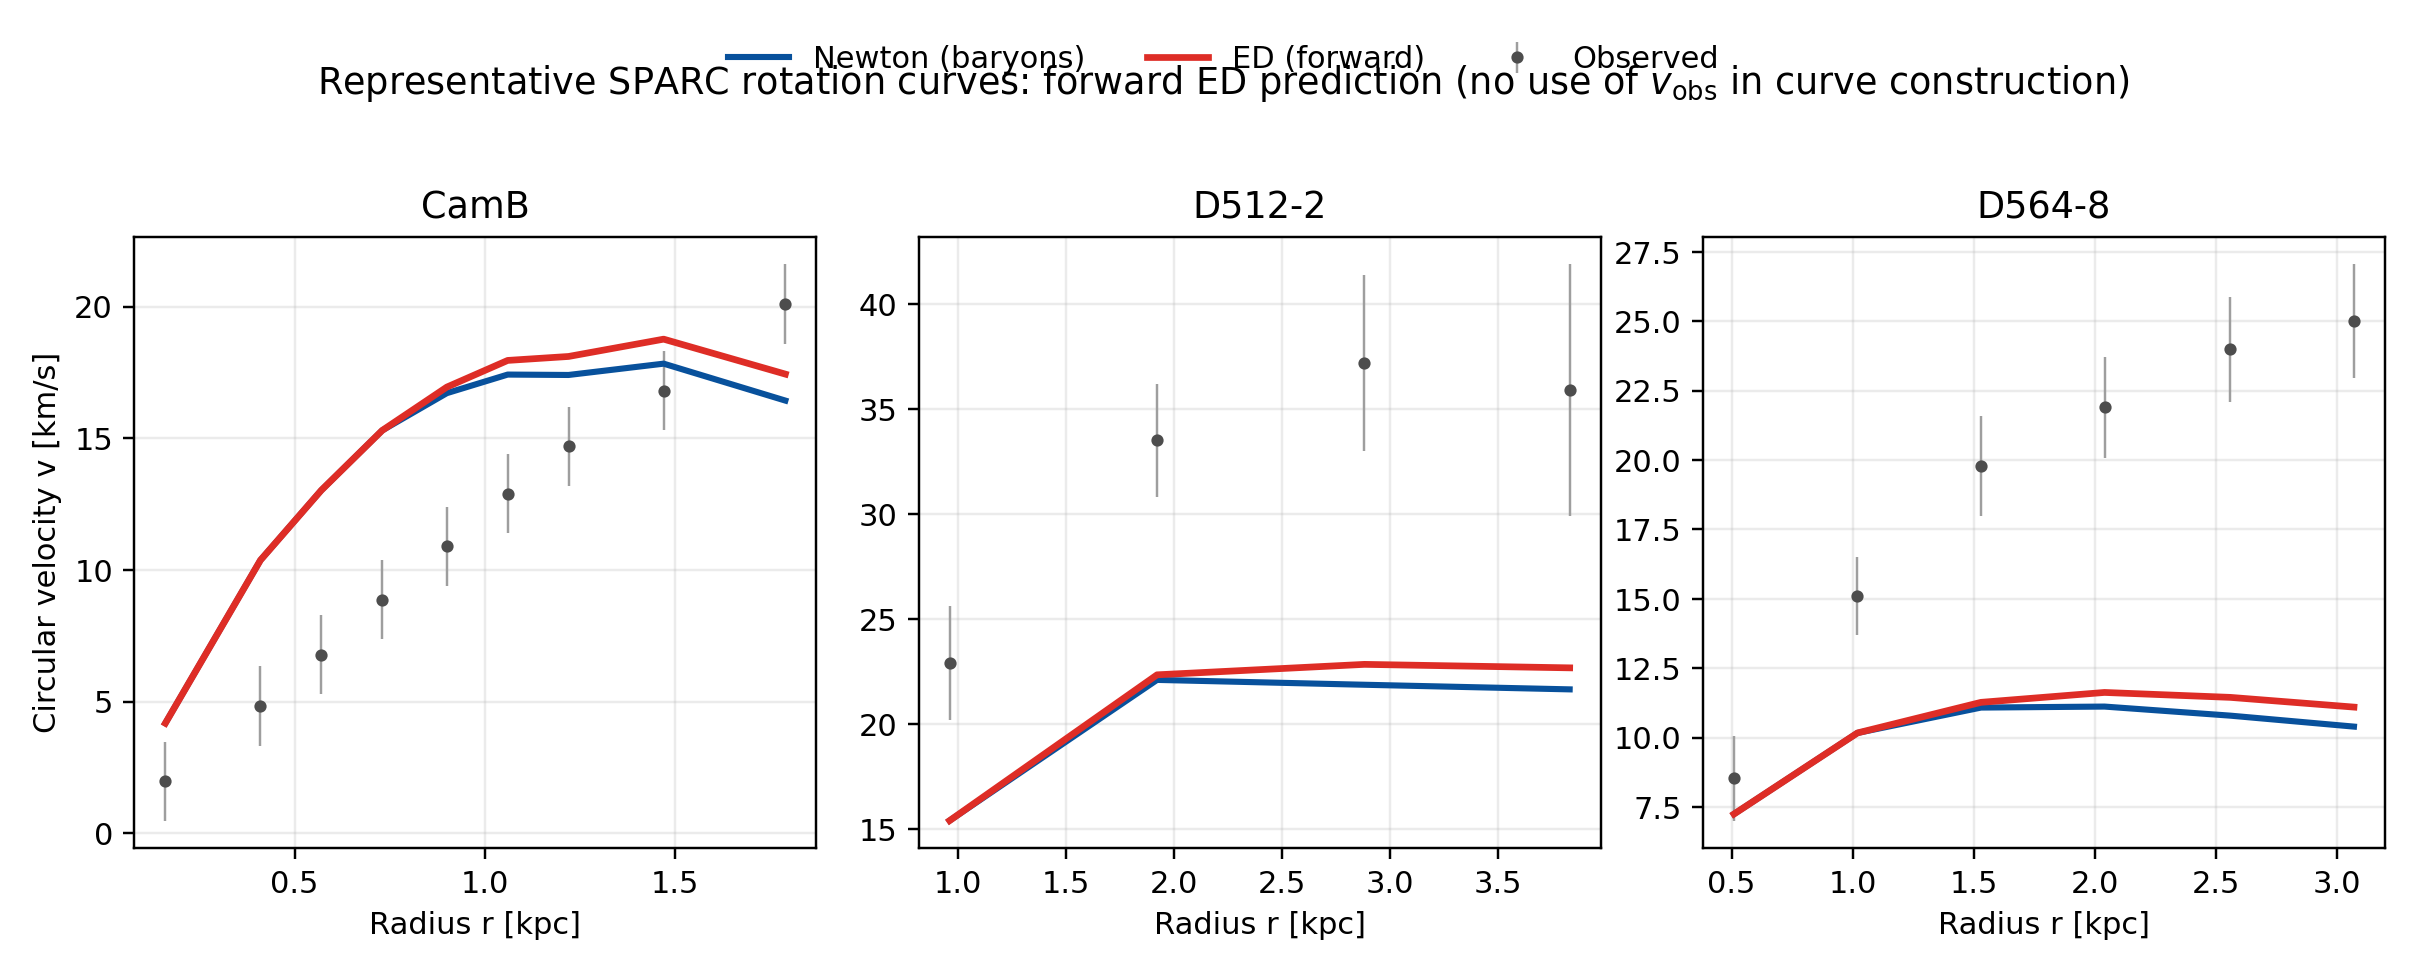
\includegraphics[width=\textwidth]{sparc_rotation_curves_forward.png}
 \caption{Representative SPARC curves.  The model curve is forward-evaluated
 from baryonic inputs after the global readout parameters have been calibrated
 on the full sample; observed velocities are overlaid for evaluation.}
 \label{fig:sparc}
\end{figure*}

These numbers are reproducible performance measurements of the declared
readout.  A decisive predictive test requires freezing the complete pipeline
and evaluating galaxies not used for global parameter selection.

\section{Dictionary-dependent cosmological growth}

Under Eq.~(\ref{eq:growthdict}), a scalar-derived equation-of-state template is
inserted into a matter-plus-dark-energy background.  The standard linear growth
equation is
\begin{equation}
 D_{,NN}+\left(2+\frac{\dd\ln H}{\dd N}\right)D_{,N}
 -\frac32\Omega_m(N)D=0,
\end{equation}
with $\fsig=\sigma_{8,0}(\dd\ln D/\dd\ln a)D$.  At the three BOSS DR12 redshifts,
the stored covariance calculation gives
\begin{equation}
 \chi^2_{\rm dict}=2.266,\qquad \chi^2_{\LCDM}=2.443.
\end{equation}
Thus $\Delta\chi^2=-0.177$, a statistically negligible difference at current
precision.  The stored
high-redshift suppression, approximately $-12$ per cent near $z_{\rm cos}=1$,
is a falsifiable prediction of the \emph{composite dictionary model}, not of the
five-dimensional bulk action alone.

\section{Prediction-factory diagnostics}
\label{sec:predictionfactory}

The revised calculation is organized as a fail-closed graph of physical links:
an output is promoted only when the action, boundary data, dimensional scale,
and evaluation protocol required by the corresponding arrow are present.  Four
new checks illustrate the distinction between generating a prediction and
retrofitting a result.

\paragraph{Boundary branches.}
All four separated self-adjoint endpoint choices were solved with the same
bulk coefficients and without observational input.  The NN branch has its
exact zero mode.  Replacing only the IR condition gives an ND lightest mode
\begin{equation}
 \mu_{\rm ND,0}=0.00274498,\qquad
 \beta_{\rm UV,0}=0.05429095.
\end{equation}
An independent continuous-shooting calculation gives
$\mu_{\rm ND,0}=0.0027447613$, a relative difference
$7.84\times10^{-5}$.  The former zero mode is therefore ultralight rather than
removed.  DN and DD start at $\mu=0.91382$ and $1.23053$, respectively, but an
exact UV point probe obeys Dirichlet data and decouples.  No branch is selected:
that requires a boundary or junction action fixed before testing.

The minimal positive Robin boundary-potential family makes one candidate
action explicit, with no boundary kinetic terms:
\begin{equation}
 Q[f]=\int\dd u\,p(f')^2+b_{\rm UV}f_{\rm UV}^2+b_{\rm IR}f_{\rm IR}^2,
 \qquad b_{\rm UV},b_{\rm IR}\geq0 .
 \label{eq:robinfamily}
\end{equation}
It implies $-p f'_{\rm UV}+b_{\rm UV}f_{\rm UV}=0$ and
$p f'_{\rm IR}+b_{\rm IR}f_{\rm IR}=0$.  The dimensionless scan coordinate is
$\rho_i=b_i/C_p$, where
$C_p=(\int\dd u/p)^{-1}=6.8836329\times10^{-4}$.  A prospective two-parameter scan
finds that IR stiffness alone cannot raise the lightest mode above
$\mu_0=0.002744976$.  UV stiffness raises that mass continuously.  At much
larger stiffness the first pair undergoes an avoided crossing and exchanges
UV residue near $\rho_{\rm UV}\simeq1.12\times10^5$; the minimum sampled
first-pair gap is $0.0119229$.
The independently finite-differenced identity
\begin{equation}
 \frac{\partial\mu_n^2}{\partial b_{\rm UV}}
 =f_n(u_{\rm UV})^2=\frac{3\beta_n^2}{I_g}
 \label{eq:robinhf}
\end{equation}
is the Hellmann--Feynman link between boundary stiffness, pole motion, and
material residue.  The map makes the consequences of any prospectively
selected boundary coefficients falsifiable; it does not select them.

\paragraph{Retrospective SPARC split.}
A deterministic galaxy-level split assigns 122 galaxies to training, 26 to
validation, and 27 to test.  The present trace-backed P5 formula was refitted
on training galaxies only; validation and test were then read once.  On the
test group (621 velocity points), its diagonal $\chi^2$ per point is 203.26
versus 254.30 for baryons-only Newton, and P5 wins in 22/27 galaxies.  A
galaxy-cluster bootstrap nevertheless gives a 95 per cent interval
$[-15.26,81.65]$ for the P5-minus-Newton log-likelihood improvement per point,
which crosses zero.  A one-global-parameter radial-acceleration relation
\citep{McGaugh2016}, fitted on the same training split, obtains
$\chi^2/{\rm point}=60.99$; P5 wins only 8/27 and its relative log-likelihood
per point is $-71.13$ with interval $[-199.42,-7.72]$.  Moreover, the P5
optimizer exhausted its fixed budget and four parameters reached their search
bounds.  All three models use the same historical unsigned baryonic
quadrature, so their comparison is aligned, but the very large absolute
$\chi^2$ values and previously exposed catalogue make this a retrospective
development diagnostic rather than confirmation.

\paragraph{Published DESI DR1 entries.}
Four published ShapeFit-plus-BAO marginal entries inside the frozen trace
domain, at $z_{\rm eff}=\{0.30,0.51,0.71,0.92\}$, were evaluated without
refitting \citep{DESI2025}.  Comparing their quoted $f\sigma_{s8}$ marginals
directly with the frozen $f\sigma_8$ curves gives
\begin{equation}
 \begin{aligned}
  \chi^2_{\rm dict,diag}&=2.6917,&
  \chi^2_{\LCDM,\rm diag}&=2.4189,\\
  \Delta\chi^2&=+0.2729.&&
 \end{aligned}
\end{equation}
Both curves are compatible with this low-dimensional diagnostic and the small
positive difference does not favour the dictionary curve.  Because distances,
shape-slope information, and within-vector and cross-bin correlations are not
modeled, these numbers are explicitly not the official DESI likelihood.

\paragraph{Wilson route.}
The new analyser validates SU(3) link matrices and implements rectangular
$W(R,T)$, effective potentials, Creutz ratios, blocking, and jackknife
uncertainties.  It fails closed on the current inputs: the available lattice
files contain plaquette/correlator summaries, not link configurations.
Consequently neither $a^2\sigma$ nor a continuum string tension is reported.

\begin{figure*}
 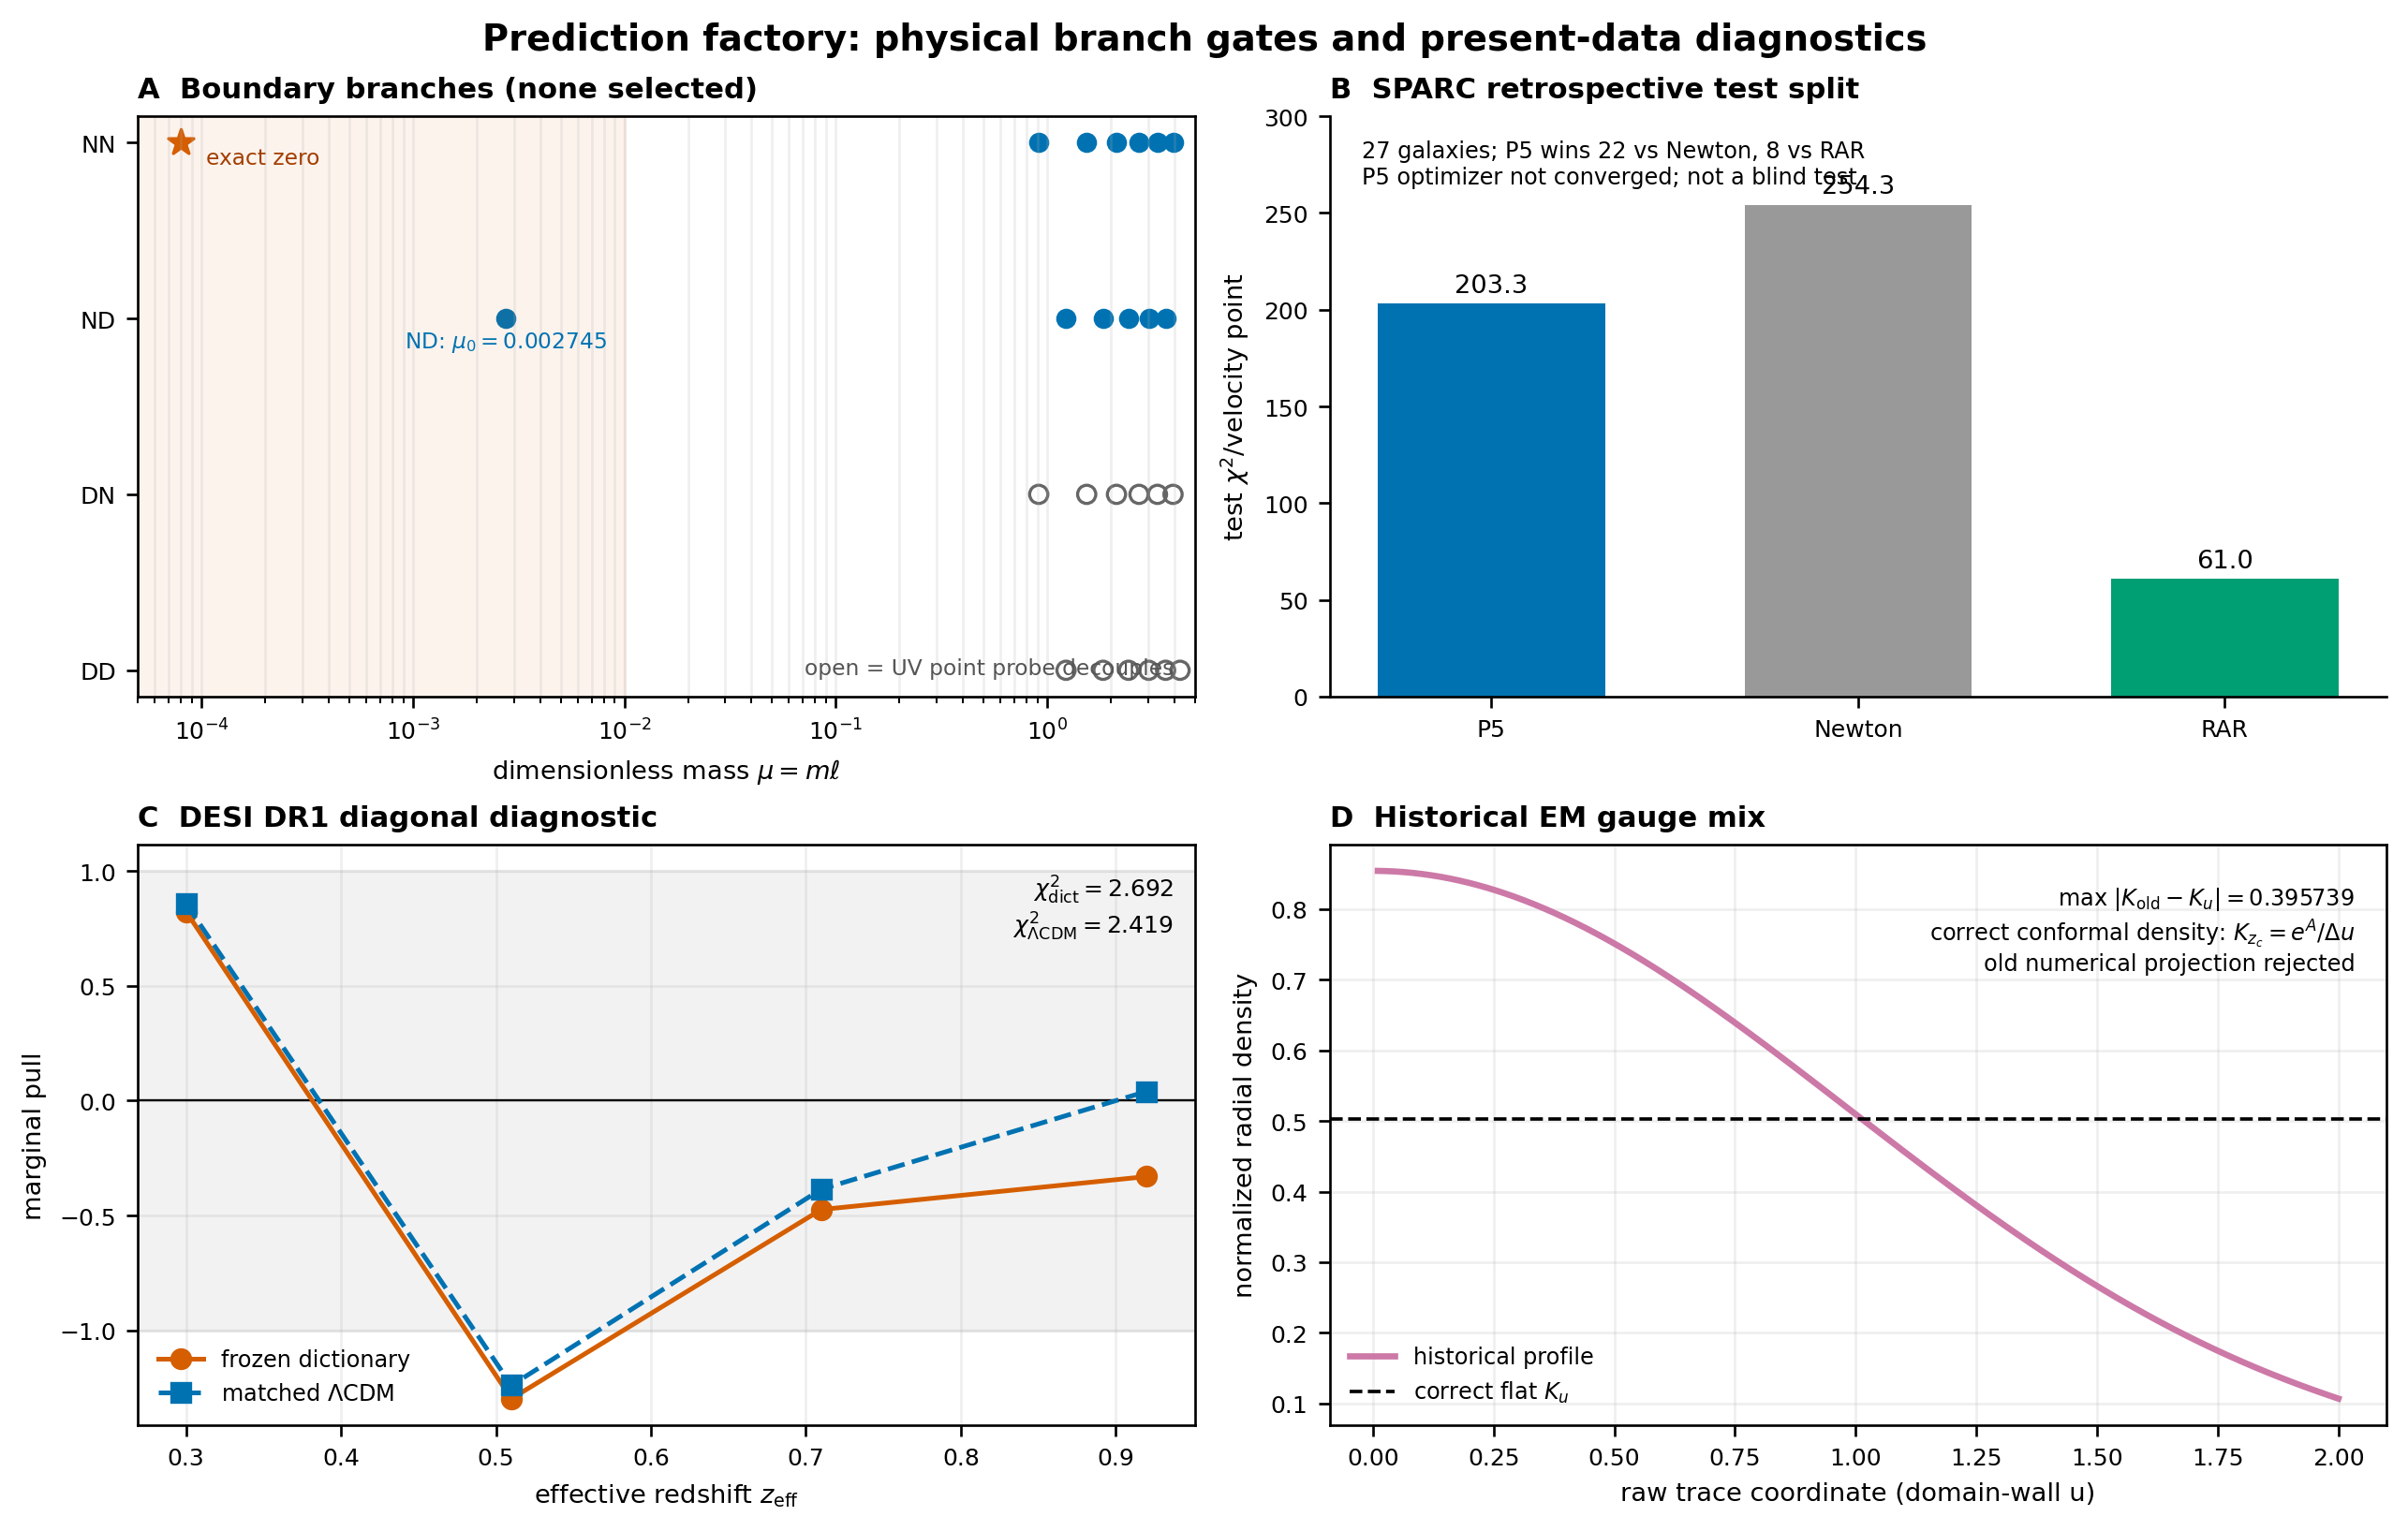
\includegraphics[width=\textwidth]{fig_prediction_factory.png}
 \caption{Prediction-factory diagnostics.  (A) The four endpoint branches:
 filled markers couple to the declared UV point probe, while open markers
 obey UV Dirichlet data; no branch is selected.  (B) Absolute SPARC test-split
 scores show that P5 improves on baryons-only Newton but underperforms the
 train-fitted RAR comparator.  (C) Published DESI DR1 marginal pulls give no
 preference over matched $\LCDM$.  (D) The historical electromagnetic profile
 is compared with the coordinate-correct $Z=1$ domain-wall zero-mode density;
 their disagreement exposes the old radial-gauge substitution.}
 \label{fig:predictionfactory}
\end{figure*}

\section{Single-arm response-operator spectroscopy}

Let $\{\psi_n\}$ denote the stored response-operator basis and let
$\delta a$ be a vector of modal amplitudes.  Each observational arm $\alpha$
has a versioned response operator
\begin{equation}
 J^{(\alpha)}_{in}=\frac{\partial y_i^{(\alpha)}}{\partial a_n},
 \qquad \delta y^{(\alpha)}\simeq J^{(\alpha)}\delta a.
\end{equation}
The DESI example reconstructs a bounded $\delta G$ from one residual vector.
This is an operational single-arm inverse problem, not a simultaneous
multi-arm detection.
This stored basis is not identified with the independently normalized
trace-carrier modes $f_n$ of Section~\ref{sec:probe}.

\begin{figure}
 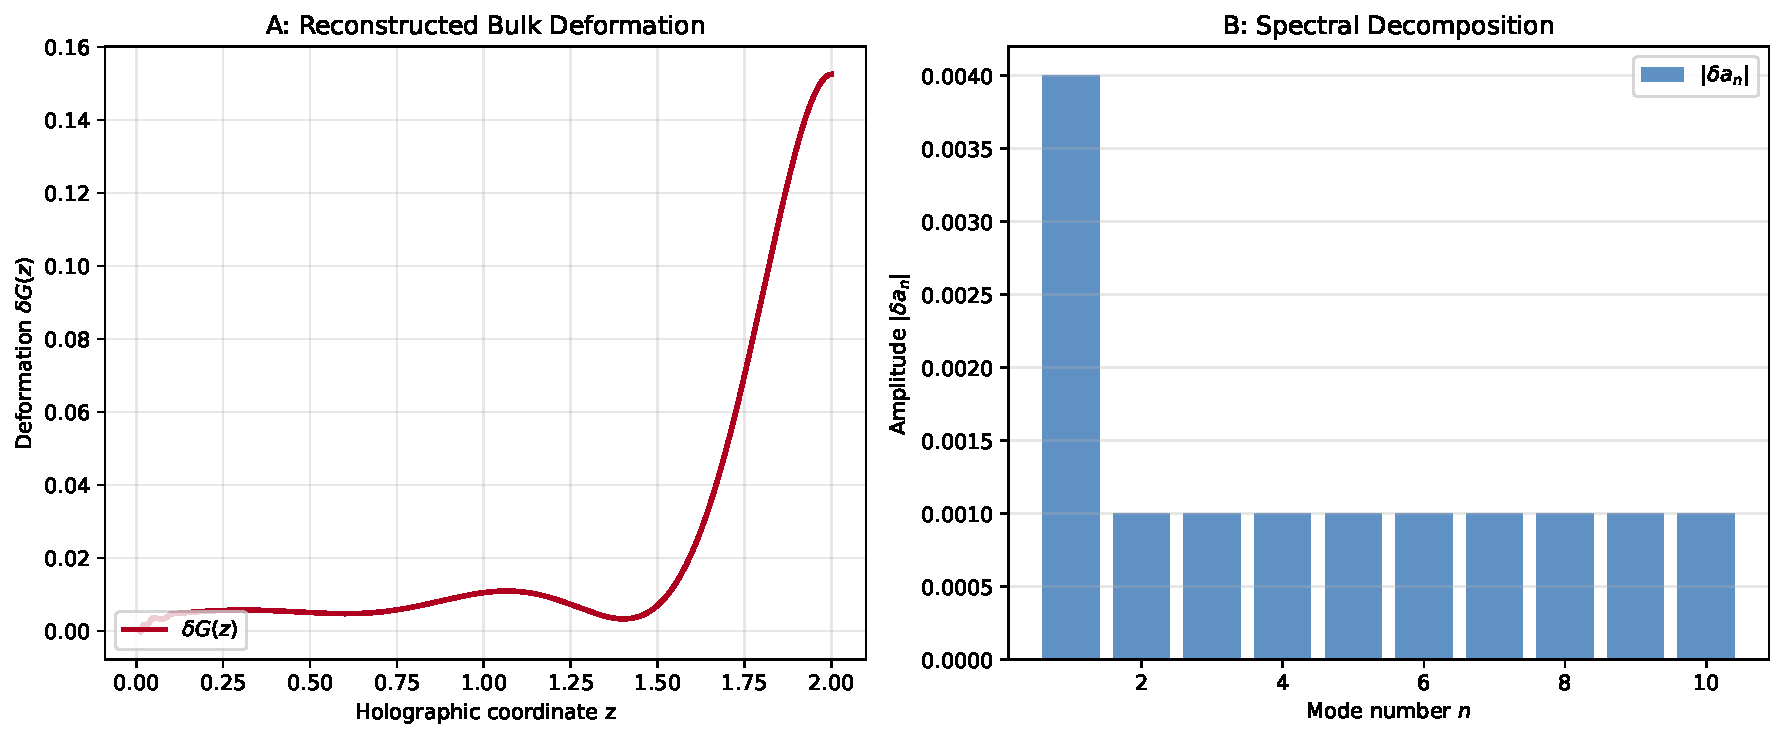
\includegraphics[width=\columnwidth]{fig_spectroscopy.pdf}
 \caption{Bounded single-arm reconstruction and modal amplitudes.  The plotted
 deformation is response-operator dependent.}
 \label{fig:spectroscopy}
\end{figure}

For diagnostic comparison, normalized arm blocks are stacked and decomposed as
\begin{equation}
 \widehat J_{\rm multi}=U\Sigma V^T,
\end{equation}
after Frobenius-per-output scaling.  The singular values summarize shared
sensitivity directions; they are not a global reconstruction.

\begin{figure}
 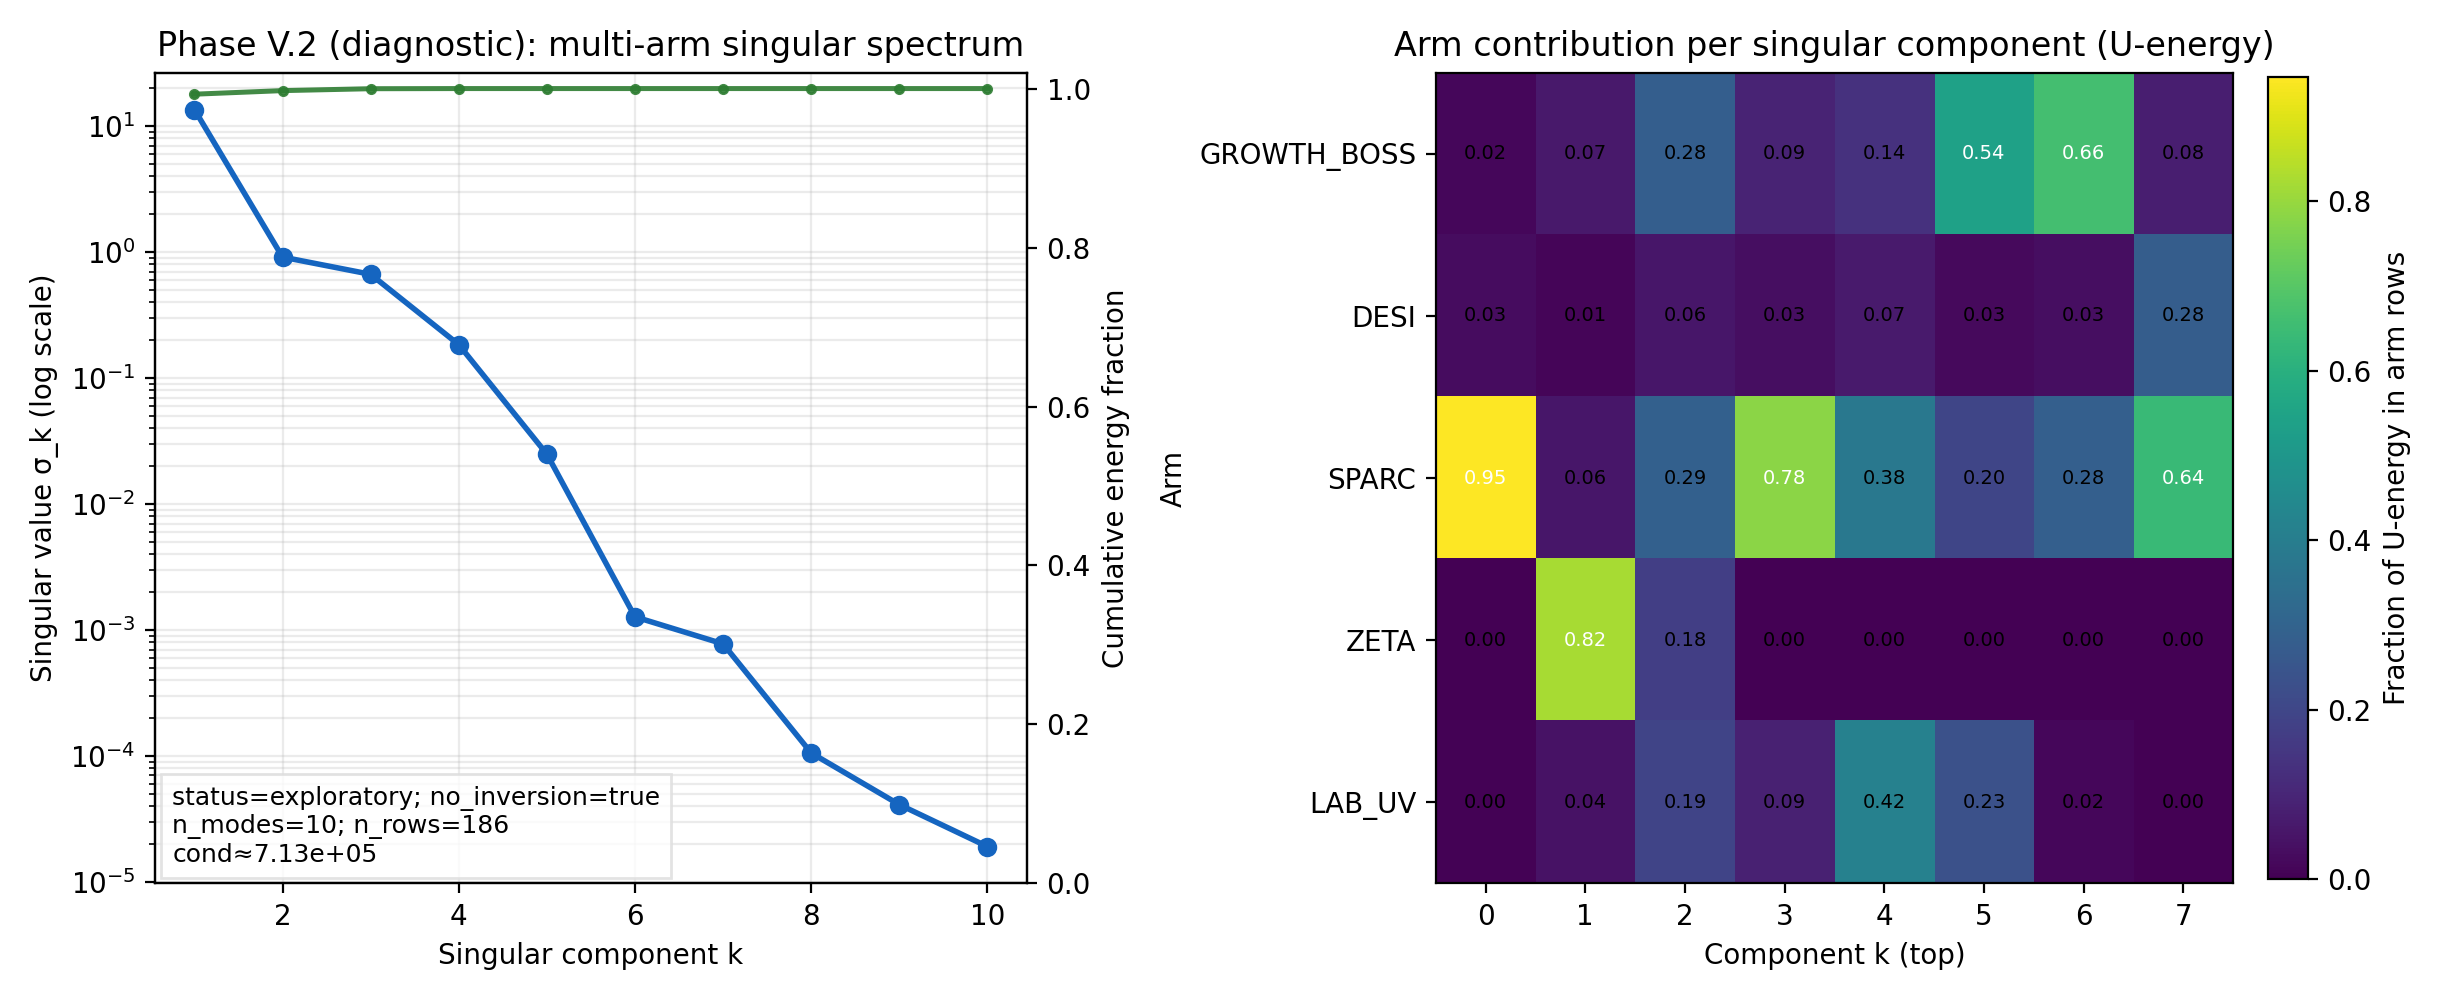
\includegraphics[width=\columnwidth]{multiarm_svd_diagnostic.png}
 \caption{SVD of the stacked normalized response blocks.  Diagnostic only; no
 cross-arm closure is inferred.}
 \label{fig:svd}
\end{figure}

\begin{figure*}
 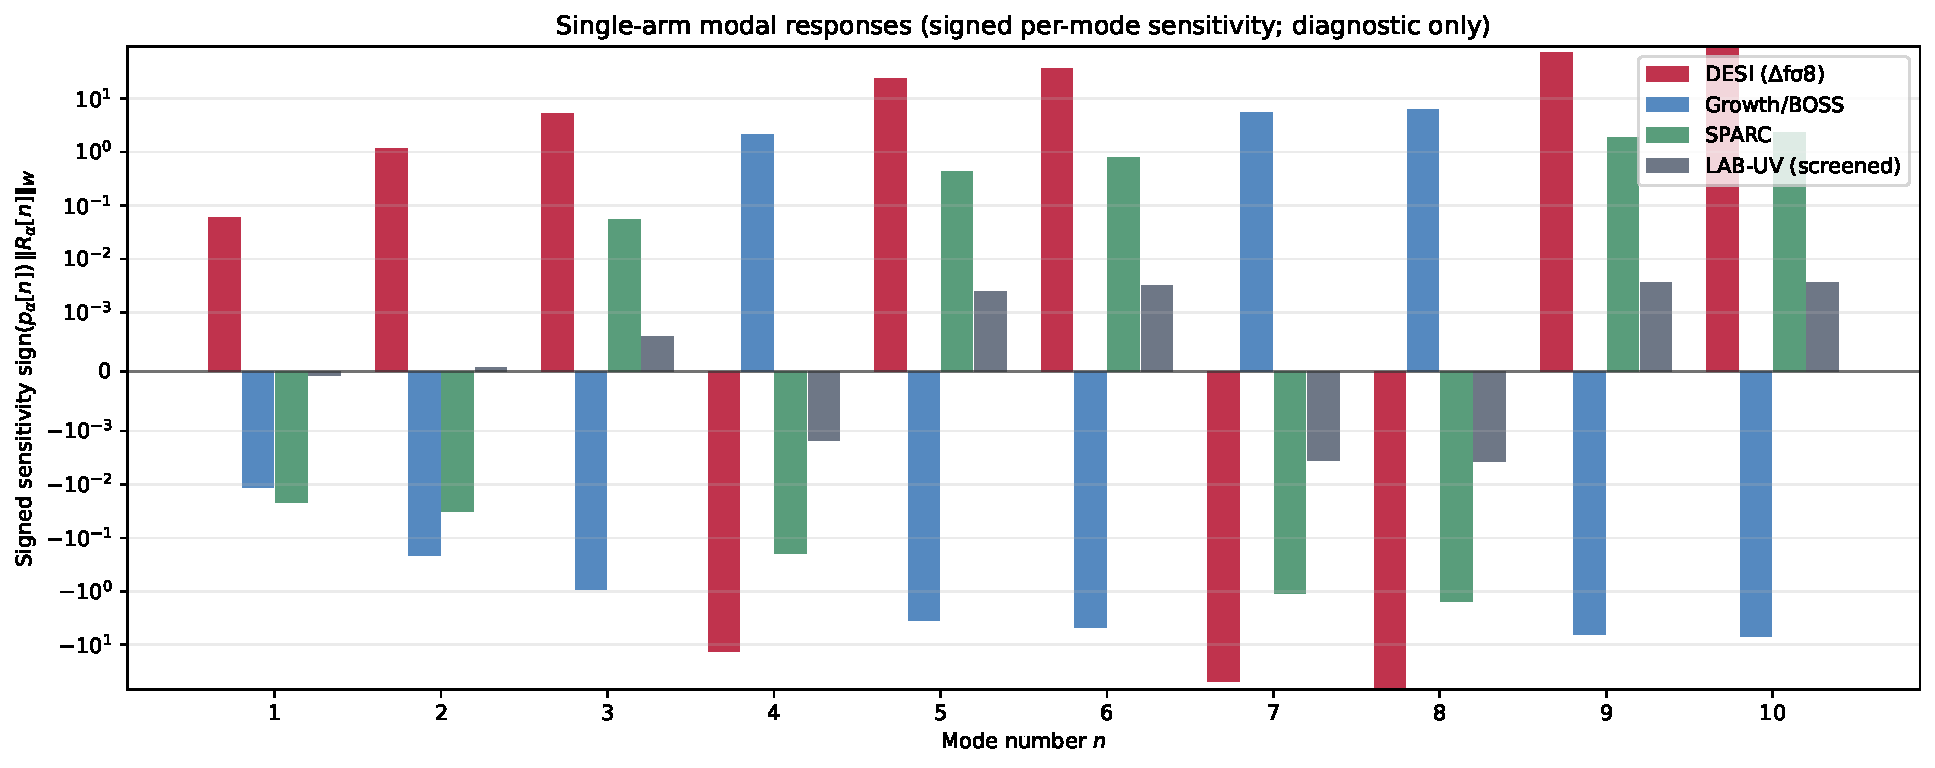
\includegraphics[width=\textwidth]{fig_single_arm_modal_responses.pdf}
 \caption{Signed per-mode sensitivities for the separate response arms.  The
 UV-screened laboratory arm remains strongly suppressed.}
 \label{fig:modal}
\end{figure*}

A modeled time dependence may be written
\begin{equation}
 \dot a_n=\sum_m M_{nm}a_m+S_n,
\end{equation}
where both $M$ and the closure source $S$ must be recorded.  Observable
projections such as $\Delta f=\sum_n\kappa_na_n$ remain conditional on their
declared coupling ansatz.

\section{Dictionary-based geometric clock and legacy laboratory interface}

The five-dimensional domain-wall curvature is
\begin{equation}
 R_{5,\rm phys}=\frac{\widehat R_5}{\ell^2},\qquad
 \widehat R_5=-8A''-20A'^2
 =\frac12\chi'^2+\frac53V.
\end{equation}
A fresh audit verifies the second, independent Einstein-trace identity to
$2.84\times10^{-14}$ and reproduces the same scalar pointwise after transforming
to conformal radial coordinates.  It also finds that the stored clock evaluated curvature
by treating the solver field $(dA)_{\rm stored}$ as $A'$, although the reproduced
trace satisfies $A'=u(dA)_{\rm stored}$.  On their common certified slice the
stored curvature spans $-21.60$ to $-19.09$, while the corrected value spans
$-13.25$ to $-73.47$; their rms difference is 26.91.  The old plot below is
retained solely as provenance.

A corrected geometry-only protocol factor can instead be declared as
\begin{equation}
 g_R(u)=\frac{e^{A(u)}\sqrt{|\widehat R_5(u)|}}
 {e^{A_0}\sqrt{|\widehat R_{5,0}|}},\qquad
 \Theta_R(u)=\int_1^u g_R(s)\dd s.
 \label{eq:clockdict}
\end{equation}

\begin{figure}
 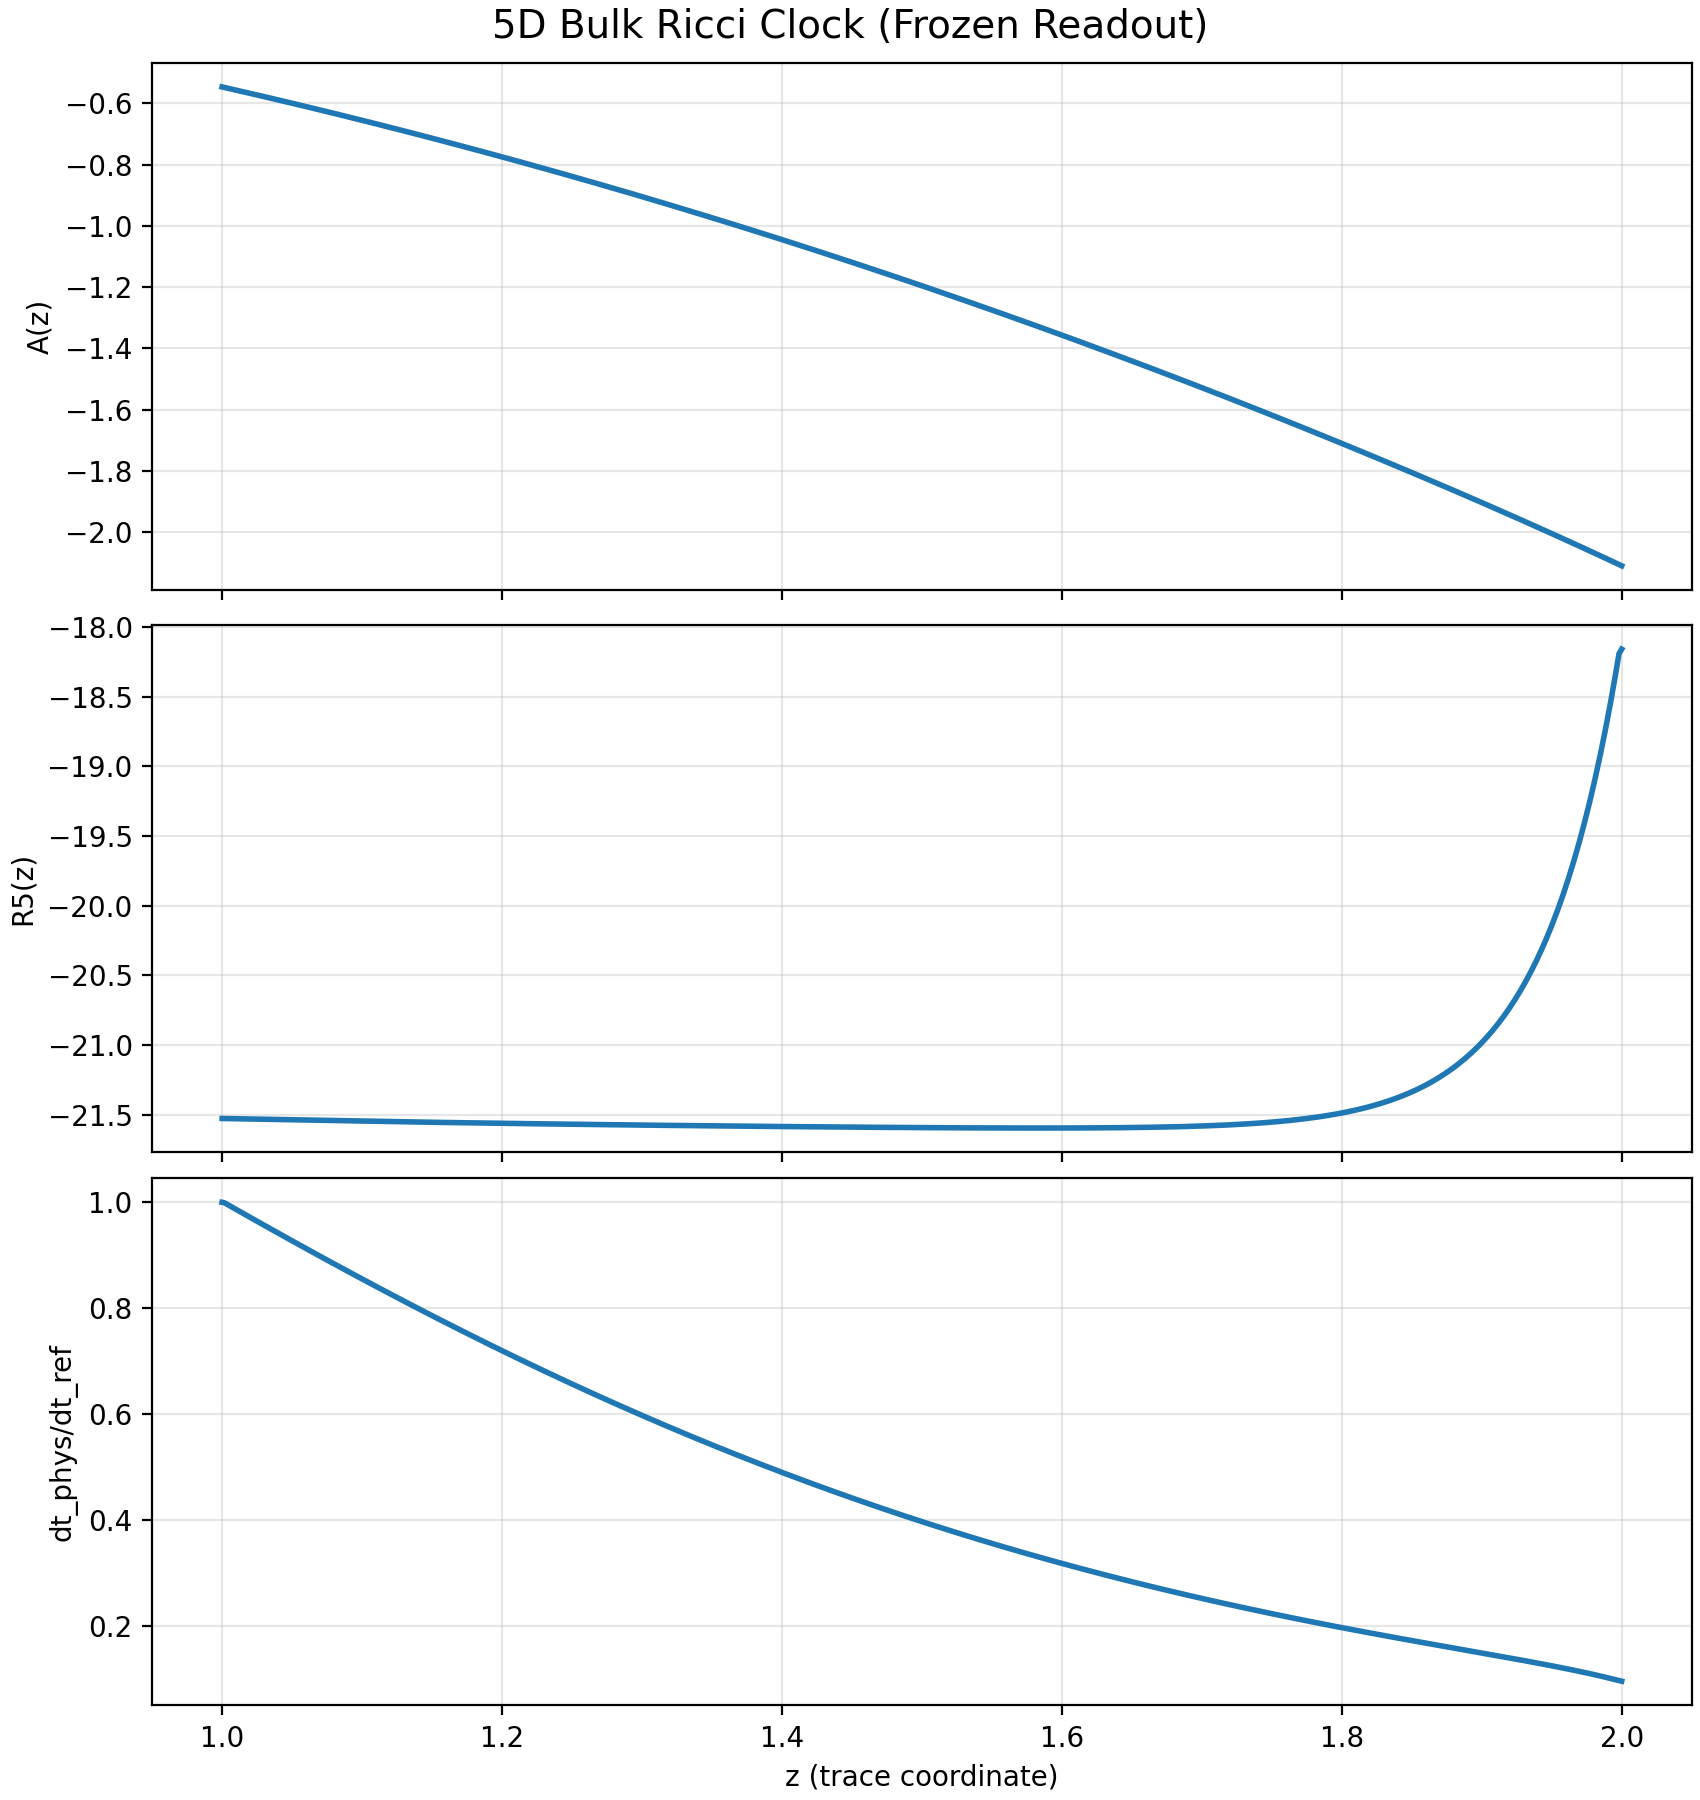
\includegraphics[width=\columnwidth]{bulk_clock_5d.png}
 \caption{Legacy warp, curvature, and protocol artefact, retained for
 provenance.  Its curvature used the mislabeled stored derivative and is not
 the corrected $\widehat R_5$ of Eq.~(\ref{eq:clockdict}).}
 \label{fig:clock}
\end{figure}

Equation~(\ref{eq:clockdict}) is a deterministic dimensionless curvature phase,
not proper time and not a mode amplitude.  On a physical compact branch it
would define $\omega_R=c\sqrt{|\widehat R_5|}/\ell$, while
$\omega_n=c\mu_n/\ell$; hence $\omega_n/\omega_R$ is geometry-fixed but seconds
still require $\ell$.  The historical LOCK5 instead inferred $\xi$ from the two
frequencies it subsequently ``verified'' and mixed this bulk curvature with
$R_4\simeq8\pi G\rho/c^2$.  Its location table is therefore a circular
calibration, not a Ricci-clock prediction.

\begin{figure*}
 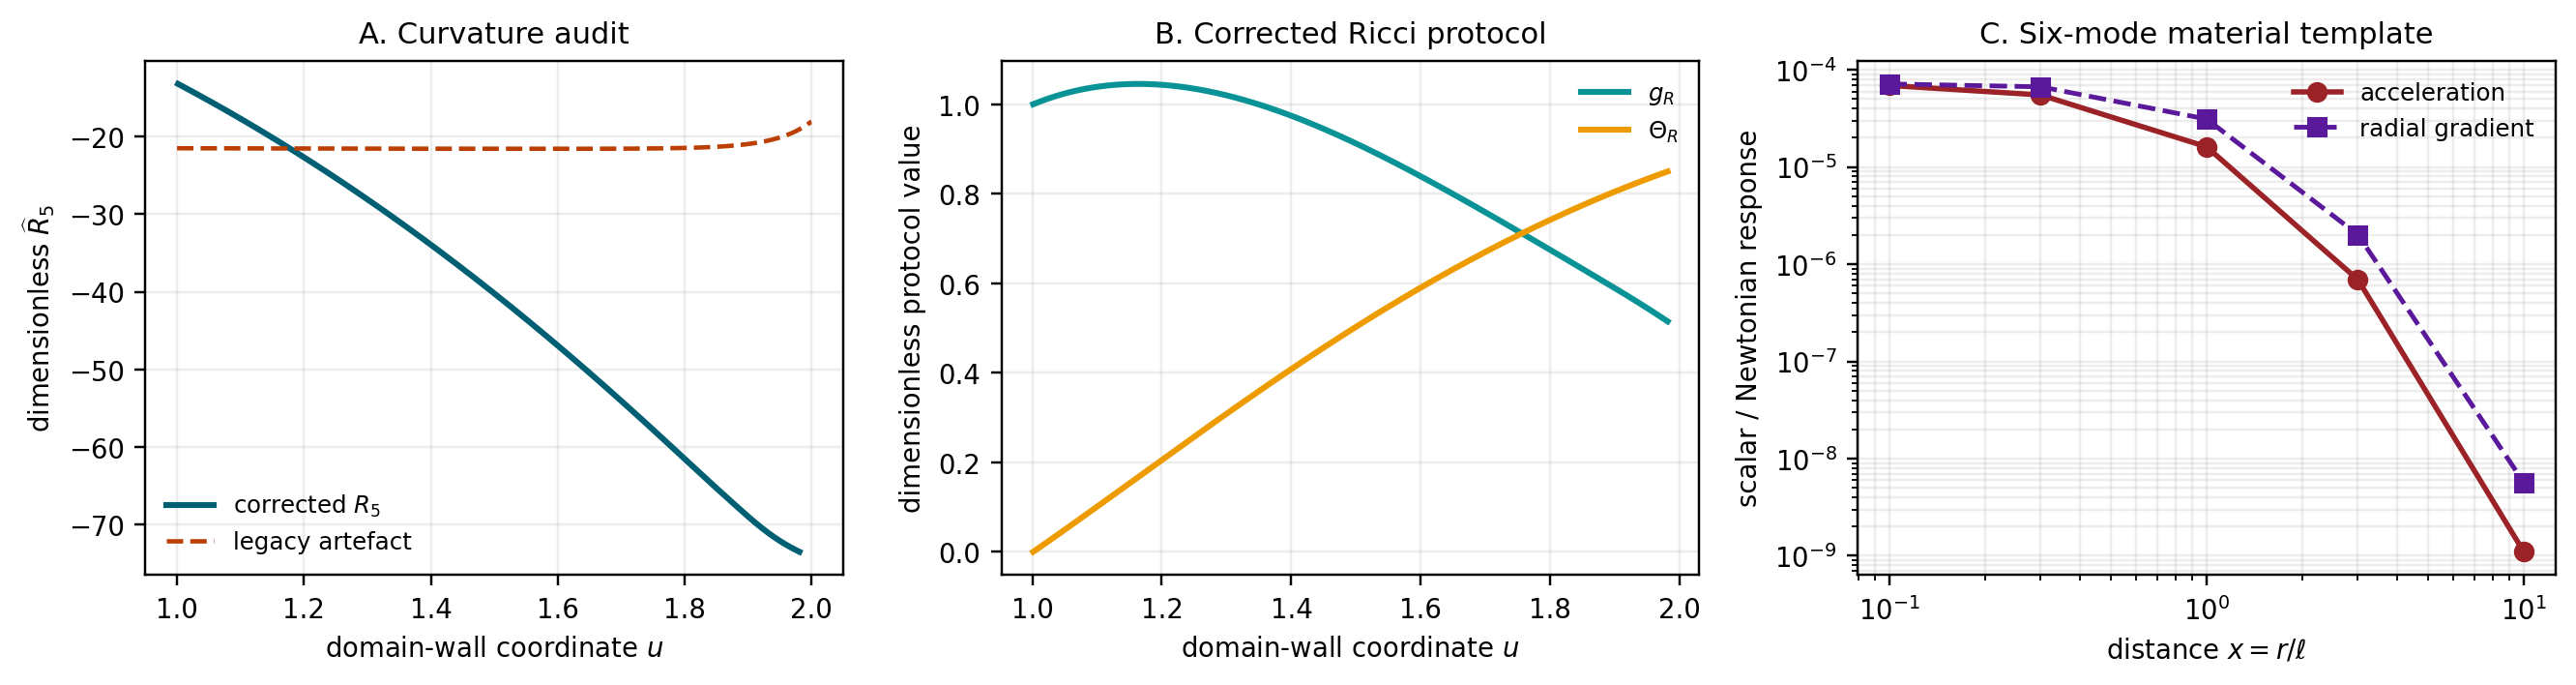
\includegraphics[width=\textwidth]{fig_ricci_material_audit.png}
 \caption{Corrected Ricci/material bridge.  Left: corrected curvature from the
 certified effective action versus the legacy series.  Centre: dimensionless
 curvature cadence and accumulated protocol coordinate.  Right: acceleration
 and tidal templates of the six positive Neumann modes; the physical horizontal
 scale remains $r/\ell$.}
 \label{fig:riccimaterial}
\end{figure*}

The historical UV-screened laboratory channel was tabulated on the raw trace
grid, labelled that grid as conformal $z$, and used
\begin{equation}
 K_{\rm old}(z)=\frac{e^{A(z)}}{\int e^{A(s)}\dd s},\qquad
 y_{\rm old}(t)=\int^{z(t)}_{z_{\rm UV}}K_{\rm old}(s)\delta(s)\dd s.
 \label{eq:legacyemkernel}
\end{equation}
The effective-action audit identifies that raw grid as domain-wall $u$.
Constructing the conformal coordinate instead requires
$\dd z_c=e^{-A(u)}\dd u$ and gives a conformal span $4.90458$, not the raw-grid
span.  For a flat photon with $Z=1$, the coordinate-correct domain-wall density
is constant, $K_u=0.507422$, whereas the historical profile differs from the
corresponding full-grid constant by as much as $0.395739$.  Thus the previous
near-machine-precision ``recovery'' was an identity produced by setting
$A=\log K_{\rm old}$, not a check against the reconstructed geometry.

For the stored Yb comparison ($n=595$), the historical projection gives
$\chi^2/n=22.59$ and Pearson $r=-0.0554$.  This null/poor-fit historical
comparison remains useful negative provenance, but it is not a test of the
coordinate-correct response and does not constitute a clock detection.

A consistent completion starts from the bulk action
\begin{equation}
 S_\gamma=-\frac{1}{4g_5^2}\int\dd^5x\sqrt{-g}\,
 Z(\chi)F_{MN}F^{MN}.
 \label{eq:bulkmaxwell}
\end{equation}
For
$\dd s^2=e^{2A(u)}\eta_{\mu\nu}\dd x^\mu\dd x^\nu+\ell^2\dd u^2$,
the dimensionless photon eigenvalues and profiles obey
\begin{align}
 -\partial_u(e^{2A}Z\partial_u f_{\gamma,n})
   &=\mu_{\gamma,n}^2Zf_{\gamma,n},\nonumber\\
 \int\dd u\,Zf_{\gamma,m}f_{\gamma,n}&=\delta_{mn},
 \qquad m_{\gamma,n}=\mu_{\gamma,n}/\ell .
 \label{eq:photonSL}
\end{align}
In conformal gauge the same equations contain the weight $e^AZ$ and the two
normalized densities are
\begin{align}
 K_u&=\frac{Z|f_\gamma|^2}{\int\dd u\,Z|f_\gamma|^2},\nonumber\\
 K_{z_c}&=\frac{e^AZ|f_\gamma|^2}
 {\int\dd z_c\,e^AZ|f_\gamma|^2},\nonumber\\
 K_u\dd u&=K_{z_c}\dd z_c .
 \label{eq:derivedemkernel}
\end{align}
The cumulative probability measures agree to $6.27\times10^{-12}$.  Equation
(\ref{eq:derivedemkernel}) is the covariant functional form underlying the
old ansatz, but Eq.~(\ref{eq:legacyemkernel}) was not its numerical realization.

The scalar--photon vertex is also fixed at this conditional action level.  In
the same almost-radial gauge used for the trace carrier, the linear constraint
of \citet{Arutyunov2000} gives
\begin{equation}
 A_u h_{uu}=\frac14\partial_u h,
 \qquad N=\frac12h_{uu}=\frac{\partial_u h}{8A_u}.
 \label{eq:lapseconstraint}
\end{equation}
The four-dimensional conformal trace cancels from
$\sqrt{-g}F_{\mu\nu}F^{\mu\nu}$, but the radial lapse $N$ does not.  For
$Z=e^{c_\gamma\chi}$, comoving endpoints, no brane kinetic terms, and
$h=\sum_nq_nf_n$, dimensional reduction therefore gives
\begin{align}
 B_F&=1+\sum_n d_{\gamma n}\frac{\varphi_n}{M_{\rm Pl}}+\cdots,\nonumber\\
 d_{\gamma n}(c_\gamma)&=\sqrt{\frac{I_g}{3}}
 \frac{\int\dd u\,e^{c_\gamma\chi}f_n'/A_u}
 {\int\dd u\,e^{c_\gamma\chi}} .
 \label{eq:dgamma}
\end{align}
No coefficient is fitted at $c_\gamma=0$.  For the six positive NN modes,
$d_{\gamma n}=(3.94563,-2.52337,2.90124,-2.42675,2.83547,-2.44815)$.
Mode signs are conventional, while the source products
$\beta_nd_{\gamma n}$ are invariant.  The unfitted response to a nonconstant
gauge kinetic function is separately fixed by
\begin{equation}
 \left.\partial_{c_\gamma}d_{\gamma n}\right|_0
 =\sqrt{\frac{I_g}{3}}\,
 {\rm Cov}_u\!\left(\chi,\frac{f_n'}{A_u}\right).
 \label{eq:dgammaSlope}
\end{equation}

Neumann photon data at $c_\gamma=0$ give the independent dimensionless comb
\begin{align}
 \mu_{\gamma,n}&=(0,0.652597,1.301427,1.939255,\ldots),\nonumber\\
 \eta_{\gamma,n}&=(1,0.61936,0.69848,0.75808,\ldots),
 \label{eq:photoncomb}
\end{align}
where $\eta_{\gamma,n}$ is the squared UV charge residue relative to the zero
mode.  With the additional interface assumption of a conserved
four-dimensional electric current localized at the UV endpoint,
$S_J=q_5\int\dd^4x\,A_\mu(x,u_{\rm UV})J^\mu$, its minimally coupled static
template is
\begin{equation}
 V_\gamma(r)=V_{\rm Coulomb}(r)
 \left[1+\sum_{n>0}\eta_{\gamma,n}e^{-\mu_{\gamma,n}r/\ell}\right].
 \label{eq:coulombcomb}
\end{equation}
Together with the scalar masses, this is a two-sector or ``double-comb''
fingerprint tied to the same $\ell$.  For a point source in the stored sign
convention, the corresponding fine-structure response is
\begin{equation}
 \frac{\delta\ln\alpha}{U}
 =\sum_n2\beta_nd_{\gamma n}e^{-\mu_nr/\ell},
 \qquad U=\frac{GM}{r}.
 \label{eq:sourcealpha}
\end{equation}
An atomic comparison would then require
$\delta\ln(\nu_A/\nu_B)=\Delta K_\alpha\,\delta\ln\alpha$.  Equations
(\ref{eq:photoncomb})--(\ref{eq:sourcealpha}) do not predict hertz until
$\ell$, a source, atomic sensitivities, and the physical bulk-photon and scalar
boundary branches are supplied.  Moving endpoints, brane bending, or localized
kinetic terms would add boundary contributions and require a new derivation.

\begin{figure*}
 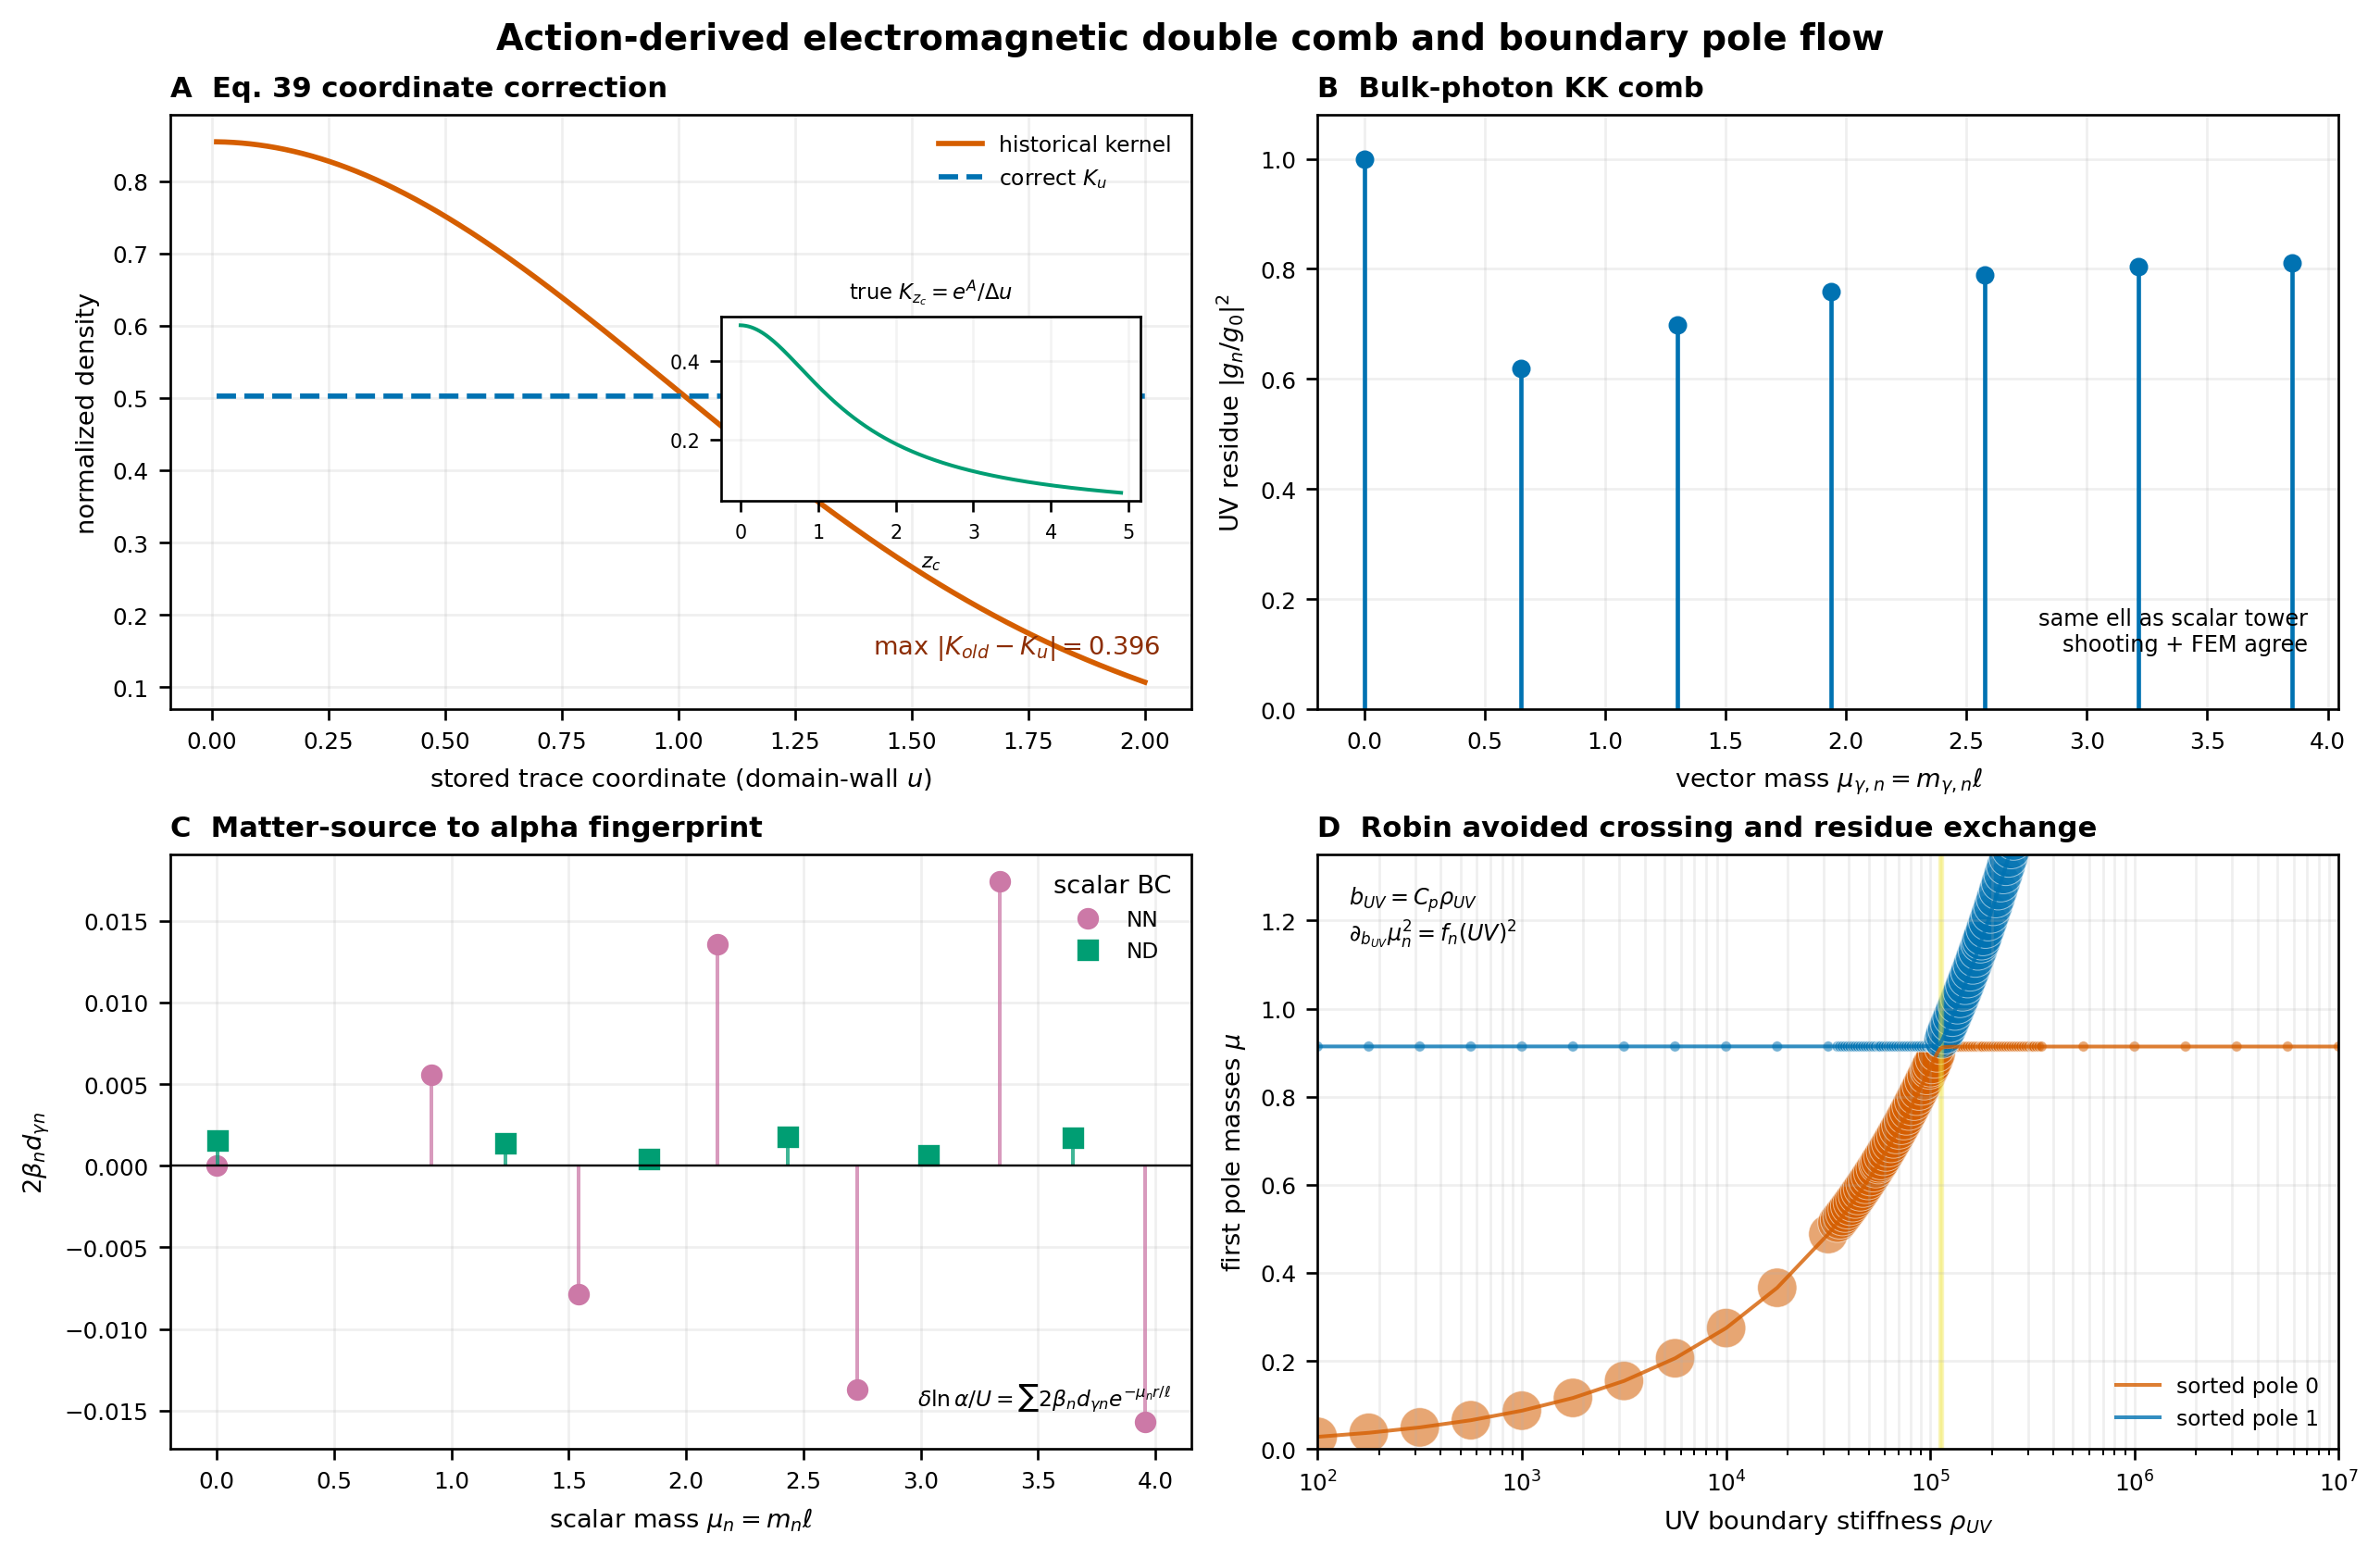
\includegraphics[width=\textwidth]{fig_em_double_comb.png}
 \caption{Coordinate-correct electromagnetic completion and double-comb
 fingerprint.  (A) The historical coordinate-mixed profile against the flat
 bulk-photon density in domain-wall gauge, with the true conformal density
 inset.  (B) Photon Kaluza--Klein masses and UV charge residues.  (C)
 Action-derived source-to-$\alpha$ coefficients for the NN and ND scalar
 branches.  (D) Robin pole motion and UV-residue exchange across the avoided
 crossing.  All axes are dimensionless; no physical boundary coefficient,
 length scale, source, atomic sensitivity, or detection is inferred.}
 \label{fig:emdoublecomb}
\end{figure*}

\begin{figure}
 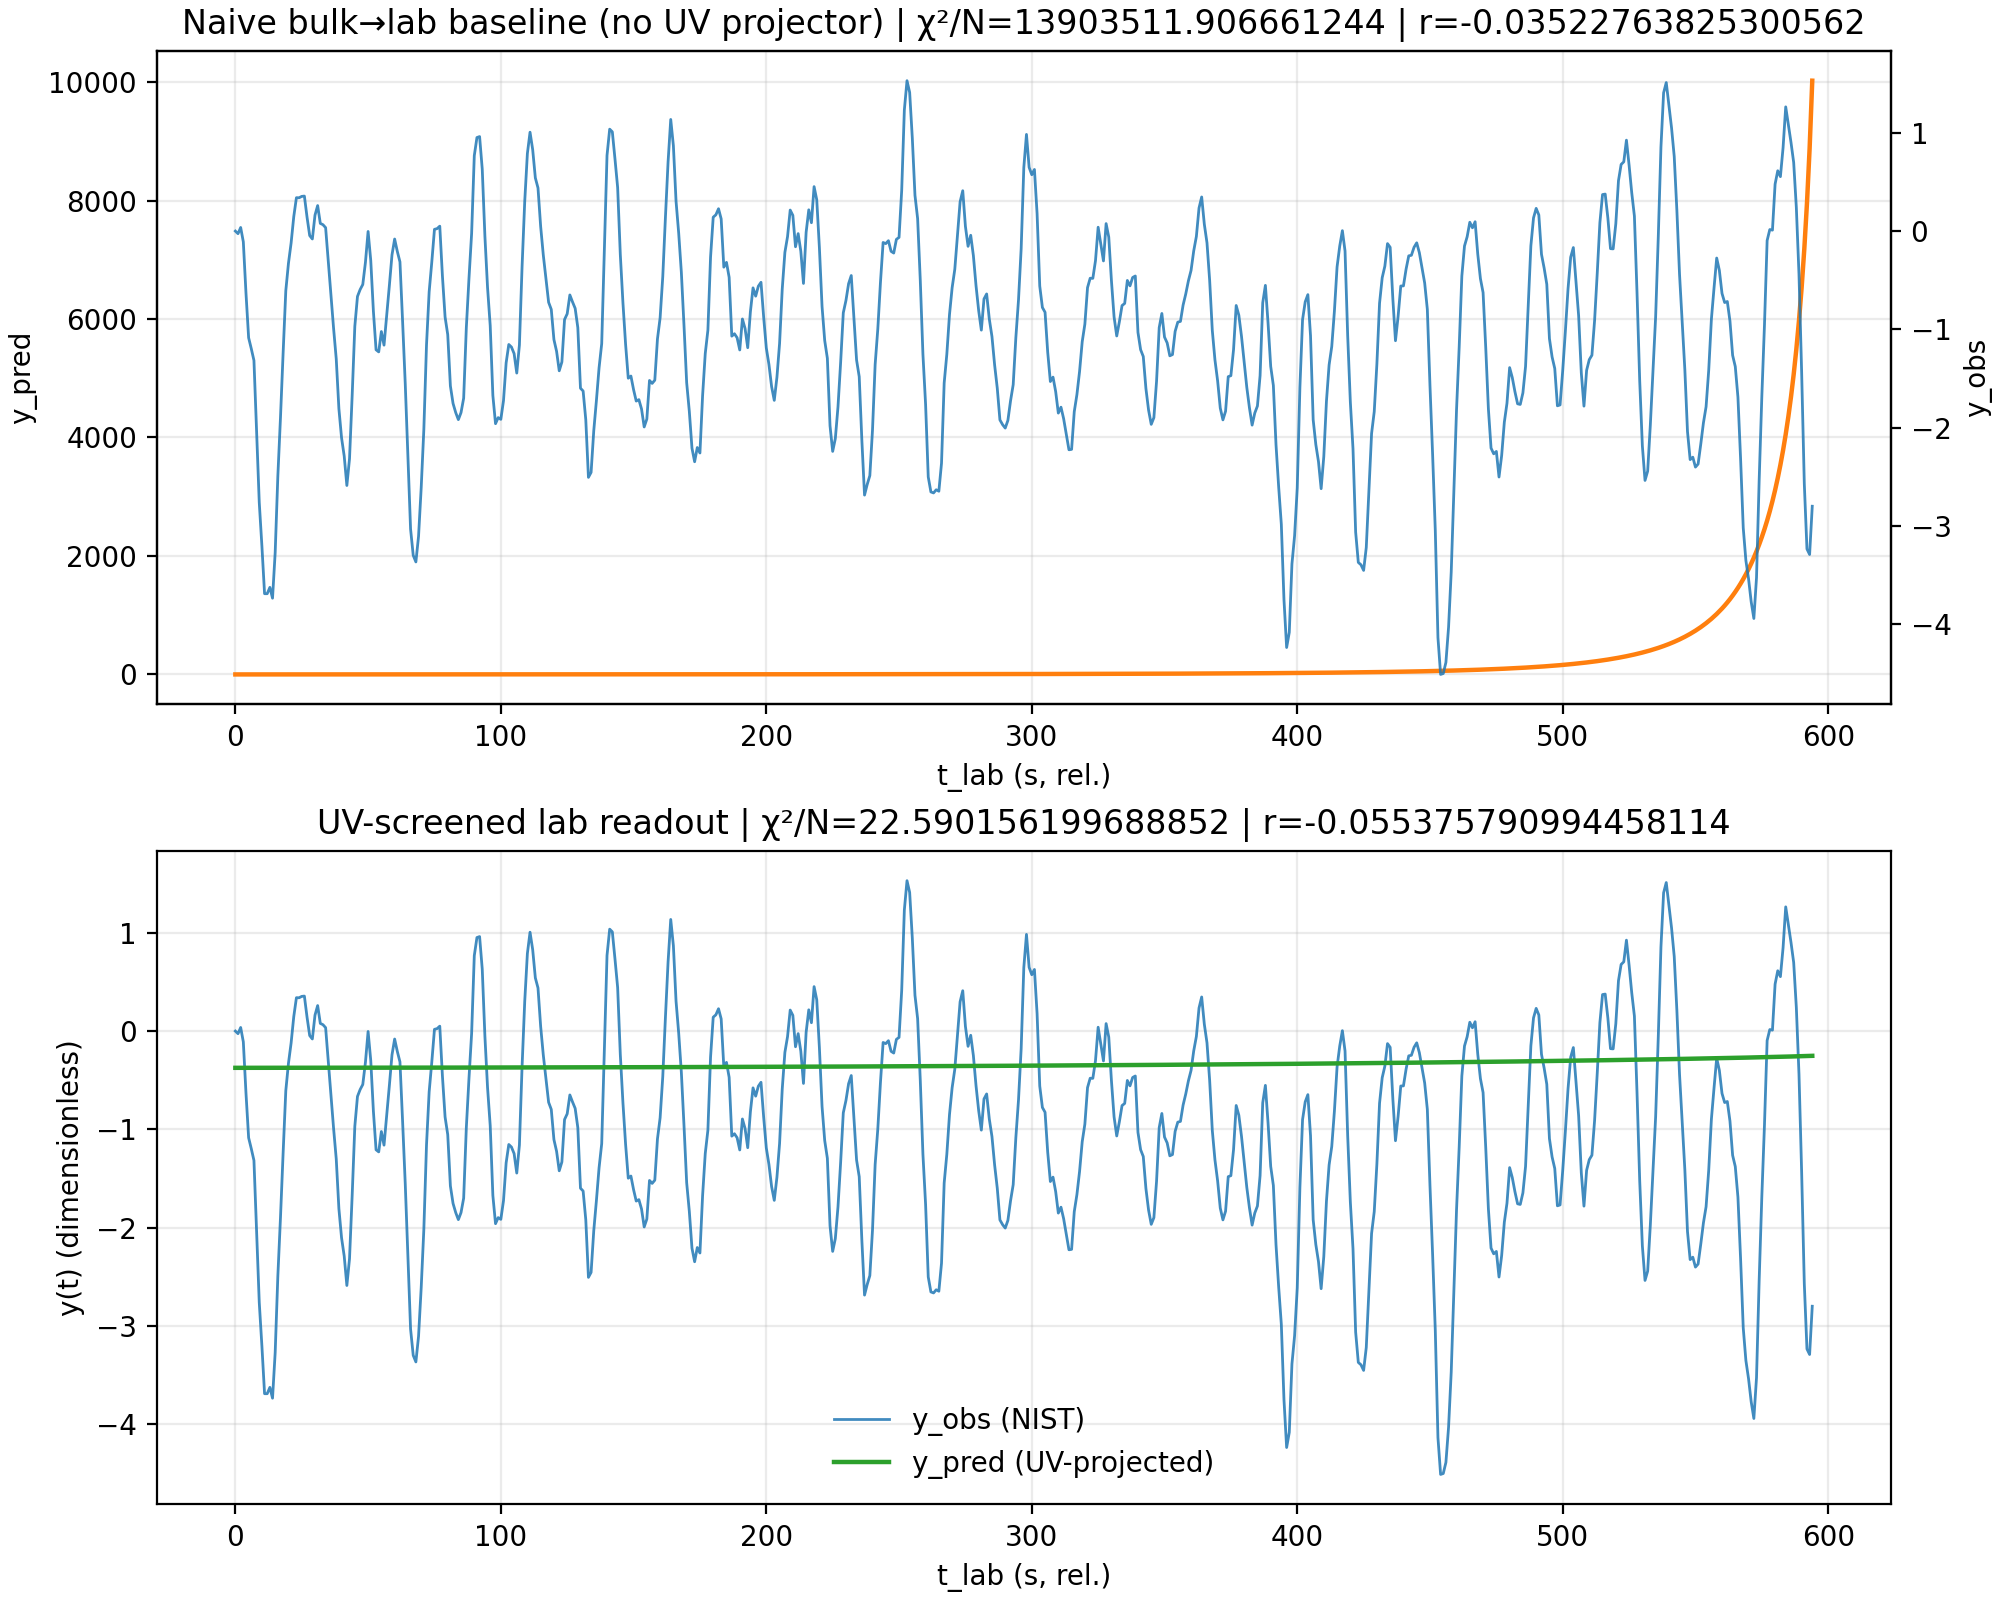
\includegraphics[width=\columnwidth]{nist_baseline_vs_uv.png}
 \caption{Historical coordinate-mixed clock projections retained for
 provenance.  Their poor correlation is not a detection and is not a test of
 the corrected bulk-Maxwell response.}
 \label{fig:nist}
\end{figure}

The Anti-Zeno response table can likewise be composed with the protocol-time
dictionary, but it remains an interface hypothesis until its action, units,
and independent calibration are specified.

\section{Discussion and validation path}

The effective reconstruction establishes a nontrivial positive result: the
actual frozen geometry admits a ghost-free Einstein--scalar completion on
the certified finite interval.  It also explains why the deformation passed
unchanged into downstream arms despite the preconditioner label error.  What it
does not do is make $K(\phi)$ and $V(\phi)$ prior predictions; they were inferred
from the achieved profiles.

A second positive result is available under a sharper evidence label.  The
compact-interval probe completion derives a normalized matter coupling without
using any observational residual or historical fitted coefficient.  Its
$\beta_0$ and mode tower are consequences of the declared interval and
Neumann benchmark, not unique consequences of the bulk geometry alone.

Several previously proposed steps are now executable rather than aspirational.
The minimal positive Robin boundary-potential family has been mapped; the electromagnetic
radial gauge has been corrected; the lapse constraint supplies a scalar--photon
vertex; the bulk photon supplies an independently checked spectral comb; and
the Wilson analysis fails closed at the missing link ensemble.  The scalar and
photon combs share one physical length and can therefore be falsified jointly
once that scale and a boundary action are fixed.  None of those calculations
selects those missing inputs.  The remaining forward programme is therefore:
\begin{enumerate}
 \item compress the tabulated $K(\phi)$ and $V(\phi)$ into a compact analytic
 form without using observational arms;
 \item freeze that action, boundary conditions, and solver tolerances;
 \item regenerate $A$, $\phi$, and the canonical $\chi$ without reading the old
 trace;
 \item derive the boundary/junction action that fixes a point in the mapped
 Robin family, and fix $\ell$ from independent physics;
 \item export thermalized SU(3) link ensembles so that the implemented
 rectangular-loop, static-potential, Creutz, and continuum pipeline can run;
 \item recompute the gauge-invariant spectrum with a confining infrared
 completion and frozen boundary conditions;
 \item compare the frozen matter force with fifth-force and post-Newtonian
 constraints without adding post-hoc screening;
 \item drive the derived material transfer law with a calibrated source and
 test it against a mechanically independent finite-element model and a held-out
 source distance;
 \item derive a four-dimensional cosmological interface before promoting the
 current radial dictionary to a growth law;
 \item choose the bulk- or brane-photon realization prospectively, including
 photon boundary data, possible localized kinetic terms, source geometry, and
 atomic response coefficients; and
 \item freeze every model and nuisance rule before an independent galaxy,
 survey-release, or clock-session holdout.
\end{enumerate}
Passing this programme would promote the current operational unification into
a forward predictive model.

\section{Conclusions}

The original work achieved a reproducible shared-background instrument: one
frozen warp geometry and deformation feed hadronic, galactic, cosmological,
laboratory, and response-operator calculations.  The revision identifies that
achievement explicitly rather than discarding it.

The previously declared canonical polynomial action and derivative labels do
not generate the frozen trace as stated.  A geometry-preserving inverse
reconstruction supplies the missing bulk completion.  Its kinetic function is
positive throughout the certified interval, its canonical representation
closes the full Einstein--scalar equations at floating-point precision, and it
recovers the operational deformation with correlation 0.999999905.

An explicitly conditional compact-interval reduction additionally produces a
matter interaction rather than merely naming one: it gives
$\beta_n=\sqrt{I_g/3}f_n$, with $\beta_0=0.0542901$ and conditional unscreened
strength $2\beta_0^2=5.89483\times10^{-3}$.  This result was obtained blind to
the observational arms and independently checked numerically.  Its physical
realization still depends on the boundary/junction completion and on the scale
$\ell$; it is neither a detection nor a unique prediction of the bulk trace.
Its Neumann massless branch is ruled out in the unscreened universal reading;
the retained positive-mode ratios and material transfer equation are therefore
a benchmark for a prospectively rederived boundary completion, not permission
to delete only the failed zero mode after comparison.
The endpoint audit sharpens that warning: the simplest IR-Dirichlet change
leaves a strongly coupled ultralight mode, while UV-Dirichlet branches make the
declared point probe vanish.  The minimal positive Robin phase map adds a stronger
result: positive IR stiffness alone has an ultralight ceiling, while UV
stiffness moves both poles and residues through an avoided crossing according
to the verified Hellmann--Feynman identity.  A boundary action, rather than
observational performance, must choose the physical realization.

The Ricci and Wilson audits close two further provenance gaps.  The corrected
$\widehat R_5$ supplies a dimensionless curvature cadence but not laboratory
seconds, and the old Wilson-labelled number is an Einstein-frame endpoint
conversion with external $\alpha'$, not a world-sheet or lattice area law.
Using a QCD scale as a compactification length would require a new UV matching
relation and cannot be inferred by chaining the present files.

The electromagnetic audit supplies a constructive bridge and one necessary
correction.  The functional conformal density
$K_{z_c}\propto e^A Z(\chi)|f_\gamma|^2$ follows from a bulk Maxwell action,
but the historical numerical profile mixed the domain-wall and conformal
coordinates.  The corrected reduction gives an invariant measure, the
action-derived coefficients $d_{\gamma n}$, and a bulk-photon Kaluza--Klein
comb.  Its shared $\ell$ with the scalar tower defines a correlated double-comb
target rather than two freely aligned spectra.  A brane-localized photon gives
a different classical result, and neither branch has yet been selected.

The scalar ratio, SPARC performance, BOSS comparison, DESI marginal diagnostic,
and UV clock projection remain reproducible outputs.  They are now labelled
according to what the current evidence establishes.  The new retrospective
SPARC split is better than a weak Newtonian comparator but worse than the
one-parameter RAR comparator; DESI gives no statistical preference; and the
Wilson route correctly reports missing input rather than manufacturing a
string tension.  This sharper separation converts an overextended single-action
claim into an executable, falsifiable research programme while preserving the
substantial computational structure already built.

\section*{Data and code availability}

The machine-readable verification bundle is available at
\url{https://github.com/RAPIDENN/HOLO_runner} and archived under
\href{https://doi.org/10.5281/zenodo.18224589}{doi:10.5281/zenodo.18224589}.
The effective reconstruction certificate, tabulated action, sealed audit, and
exact control flow are included under \path{first_principles_audit/}.  The
conditional interaction, its zero-input declaration, finite-element spectrum,
independent shooting comparison, Robin phase map, coordinate-correct
electromagnetic completion, double-comb fingerprint, Wilson input contract,
and present-data diagnostics are stored there as machine-readable artefacts.
Third-party SPARC, BOSS, Planck, DESI, and NIST data remain subject to their
original distribution policies.  The repository bundle records derived
metrics and provenance rather than redistributing restricted measurements.

\section*{Acknowledgements}

This work uses publicly released SPARC, BOSS DR12, and Planck products.  The
author thanks readers who emphasized the need for external refereeing and a
clear separation between a reusable computational instrument and a physical
detection claim.

\begin{thebibliography}{99}
\bibitem[Alam et al.(2017)]{Alam2017}
Alam S., et al., 2017, MNRAS, 470, 2617

\bibitem[Arutyunov et al.(2000)]{Arutyunov2000}
Arutyunov G., Frolov S., Theisen S., 2000, Phys. Lett. B, 484, 295--305

\bibitem[Breitenlohner \& Freedman(1982)]{Breitenlohner1982}
Breitenlohner P., Freedman D. Z., 1982, Ann. Phys., 144, 249

\bibitem[DeWolfe et al.(2000)]{DeWolfe2000}
DeWolfe O., Freedman D. Z., Gubser S. S., Karch A., 2000,
Phys. Rev. D, 62, 046008

\bibitem[Bertotti et al.(2003)]{Bertotti2003}
Bertotti B., Iess L., Tortora P., 2003, Nature, 425, 374--376

\bibitem[Damour \& Donoghue(2010)]{Damour2010}
Damour T., Donoghue J. F., 2010, Class. Quantum Grav., 27, 202001

\bibitem[DESI Collaboration et al.(2025)]{DESI2025}
DESI Collaboration et al., 2025, JCAP, 09, 008

\bibitem[Gürsoy et al.(2008)]{Gursoy2008}
Gürsoy U., Kiritsis E., Nitti F., 2008, JHEP, 02, 019

\bibitem[Gürsoy et al.(2011)]{Gursoy2011}
Gürsoy U., Kiritsis E., Mazzanti L., Michalogiorgakis G., Nitti F., 2011,
Lect. Notes Phys., 828, 79

\bibitem[Lelli et al.(2016)]{Lelli2016}
Lelli F., McGaugh S. S., Schombert J. M., 2016, AJ, 152, 157

\bibitem[McGaugh et al.(2016)]{McGaugh2016}
McGaugh S. S., Lelli F., Schombert J. M., 2016,
Phys. Rev. Lett., 117, 201101

\bibitem[Morningstar \& Peardon(1999)]{Morningstar1999}
Morningstar C. J., Peardon M., 1999, Phys. Rev. D, 60, 034509

\bibitem[Athenodorou \& Teper(2020)]{Athenodorou2020}
Athenodorou A., Teper M., 2020, JHEP, 11, 172

\bibitem[Planck Collaboration(2020)]{Planck2020}
Planck Collaboration, 2020, A\&A, 641, A6
\end{thebibliography}

\end{document}
